\documentclass[12pt]{article}
\usepackage[margin=1in]{geometry}
\usepackage {setspace} %% for line space
\usepackage[hang,flushmargin]{footmisc} %control footnote indent
\usepackage{url} % for website links
\usepackage{amssymb,amsmath}%for matrix
\usepackage{graphicx}%for figure
\usepackage{appendix}%for appendix
\usepackage{float}
\usepackage{multirow}
\usepackage{longtable}
\usepackage{morefloats}%in case there are too many float tables and figures
\usepackage{caption}
\usepackage{subcaption}
\usepackage{listings}
\captionsetup[subtable]{font=normal}
\usepackage{color}
\usepackage{hyperref}
\usepackage[utf8]{inputenc}
\usepackage{pdflscape}

\setlength{\parindent}{0em}% paragraph indention
\setlength{\parskip}{0.5em}

\graphicspath{{figure/}}


\begin{document}
%\input{Proposal_draft-concordance}
%cover page
\begin{titlepage}
\title{\normalsize Data-adaptive SNP-set-based Association Tests of Longitudinal Traits}
\date{}
\maketitle

{\normalsize
\begin{center}
by\\[5mm]
Yang Yang, M.S\\[10mm]
APPROVED:\\[10mm]
\end{center}}

\begin{table}[h]
\begin{flushright}
\begin{tabular}{ p{8cm}}

\hline
Dissertation Chair, PHD\ \\[0.8cm]
\hline
Minor Advisor, PHD\\[0.8cm]
\hline
Breadth Advisor, PHD\\[0.8cm]
\hline
External Advisor, PHD\\[0.8cm]


\end{tabular}
\end{flushright}
\label{default}
\end{table}

\thispagestyle{empty}
\pagestyle{empty}
\end{titlepage}

\newpage
\thispagestyle{empty}
\begin{center}
Coptyright\\
by\\
Yang Yang, M.S\\
2014
\end{center}


\newpage
\thispagestyle{empty}
\doublespacing
\begin{center}
DEDICATION\\
Persistent support from my family members:\\
Nainan Hei\\
\&\\
Tianpeng Yang and Qi Lu
\end{center}


\newpage
\thispagestyle{empty}
\doublespacing
\begin{center}
{\normalsize Data-adaptive SNP-set-based Association Tests of Longitudinal Traits }\\[3.2cm]

by\\[0.5cm]

Yang Yang, M.S\\[3.2cm]

Presented to the Faculty of The University of Texas\\
School of Public Health\\
in Partial Fulfillment\\
of the Requirements\\
for the Degree of\\[1.5cm]
DOCTOR OF PHILOSOPHY\\[1.5cm]
\singlespacing
THE UNIVERSITY OF TEXAS\\
SCHOOL OF PUBLIC HEALTH\\
Houston, Texas\\
November, 2014
\end{center}


\newpage
\thispagestyle{empty}
\doublespacing
\begin{center}
ACKNOWLEDGMENTS
\end{center}
Great thanks to my dissertation adviser Dr. Peng Wei, as he guided me ever from 2011, put countless efforts in training me to be a countable person, and then a qualified Ph.D. He taught me with his solid background in statistical theory, to make me an as well solid statistician to qualify for future career challenges; he corrected me many times to let me not bypass by instead overcome the difficulty in a native English style of written and oral communications; he also taught me the spirit of persistence, either in research or in life, which is indispensable to every kind of definition of success. I also want to appreciate the great helps from my dissertation committee members: Dr. Alanna C. Morrison, Dr. Yun-Xin Fu and Dr. Han Liang. They are talented experts in their fields and provided me with enormous valuable advice towards my research and writings. I also want to express my special gratitude to Dr. Han Liang. As I have been a Graduate Research Assistant in MD Anderson Cancer Center under his supervision and mentoring between 2012 to 2013, he inspired me to be a bioinformatics researcher rather than a proficient analyst, ignited me the passion in cancer genomics, influenced me to have innovative thinking and meticulous altitude in pursuing science.


\newpage
\thispagestyle{empty}
\doublespacing
\begin{center}
{\normalsize  Data-adaptive SNP-set-based Association Tests of Longitudinal Traits}\\[2.3cm]
\singlespacing
Yang Yang, M.S\\
The University of Texas\\
School of Public Health, 2014
\end{center}

\doublespacing
\noindent
Dissertation Chair, Peng Wei, PhD\\
Minor Advisor, Alanna C. Morrison, PhD\\ 
Breadth Advisor, Yun-Xin Fu, PhD \\
External Advisor, Han Liang, PhD\\



\newpage
\tableofcontents

\newpage
\listoftables

\newpage
\listoffigures
 

\newpage
%%%%%%%%%%%%%%%%%%%%%%%%%%%%%%%%%%%%%%%%%%%%%%%%%%%%%%%%%%%%
\section{Background}\label{sec:background}
%%%%%%%%%%%%%%%%%%%%%%%%%%%%%%%%%%%%%%%%%%%%%%%%%%%%%%%%%%%%
\doublespacing
% This is a template for UT SPH Phd proposal based on \LaTeX \cite{lamport1986document}.\\
Genome-wide association studies (GWASs) have been popular since 2007, and hundreds of GWASs have been published already (A Catalog of Published Genome-Wide Association Studies: http://www.genome.gov/26525384). The most popular approach in GWAS is to test the association with complex traits on single nucleotide polymorphism (SNP), also known as single nucleotide variant (SNV), one by one, then select the the SNVs that meet a stringent significance level after multiple testing correction, such as the Bonferroni and false discovery rate (FDR) methods \cite{McCarthy2008,Hirschhorn2005}. However, this strategy will suffer from low power when the minor allele frequency (MAF) of the SNV is low (between $1\%$ and $5\%$), and as a result the signals contained within the low MAF SNVs are hard to detect \cite{Sham2014}. In addition, the usual regression coefficient estimate of SNV becomes unstable due to the small number of minor allele counts and the coefficient estimate's variance becomes very large \cite{Sham2014}. It will become an even more severe problem for rare variants (RVs) analysis. RVs are usually defined as SNVs with MAF below $1\%$ \cite{Bansal2010}. In spite of their extremely low MAF, RVs' important role in conferring disease risk cannot be underestimated. Due to the constraint of purifying selection, causal and functionally deleterious variants are often RVs. In turn, they typically have larger effect sizes than common variants \cite{Fu2013,Bansal2010,Sham2014,McCarthy2008}. Therefore, developing new association tests tailored to low MAF SNVs and RVs has been a very active research area in recent years. Due to the nature of low MAF, either increasing the total sample size or aggregating information across multiple variants in an analysis set (e.g. gene) is expected to achieve a practically acceptable power \cite{Capanu2011,Basu2011,Bansal2010,Sham2014}. As increasing the sample size is usually expensive and demanding, SNP-set or Gene-set based association tests pooling together information have been the major research directions \cite{Ye2011,Pinto2010,Sham2014}. Sets of SNVs can be defined by gene boundaries (i.e., Gene-based) or sliding windows; Sets of genes can be defined by Gene Ontology terms, protein-protein interactions, canonical gene signal pathways and gene expression networks as examples. \cite{Sham2014,DelaCruz2010,Weng2011,Wang2010,Wei2012a}.

\subsection{Gene-based association tests}\label{sec:bg:Gb test}
A large number of gene-based association tests (mainly designed for RVs) have been proposed in recent years. The earliest methods include the cohort allelic sums test (CAST)\cite{Morgenthaler2007} and the combined multivariate and collapsing (CMC) method \cite{Li2008}. Afterward, more advanced tests were proposed. Those methods can be classified into major groups including:
%%%%%%%%%%%
\begin{itemize}
\item A very famous category of these methods is the so-called "burden test" or "sum test", such as a weighted sum statistic (WSS) \cite{Madsen2009}, which uses MAF based weighting scheme to combine the sum statistics from multiple SNVs in a region, with the assumption that all the alleles to be deleterious. WSS is also known as Madsen and Browning test (MB test). Many other tests within "burden test" category inherited and improved the WSS performance in some scenarios \cite{Hoffmann2010,Zhang2010,Ionita-Laza2011,Feng2011}. Such improved "burden tests" includes the sibpair and odds ratio weighted sum statistics (SPWSS, ORWSS) \cite{Zhu2010,Feng2011}; the replication-based test (RBT) \cite{Ionita-Laza2011} which is built on WSS with the aim to be less sensitive to the presence of both risk and protective effects in a genetic region of interest; the yet another weighted-sum test with a "step-up" approach to choose the 'best' combination of rare variants into a single aggregated group \cite{Hoffmann2010}; the MB test with approximately optimal collapsing (AOC) method \cite{Zhang2010}; a data-driven P-value Weighted Sum Test (PWST) \cite{Zhang2011} which used both significance and direction of individual variant effect from single-variant analysis to calculate a single weighted sum score.
%%%%% 
\item Another major category of gene-based association tests is the so-called "variance-component test", which can be formulated as testing on a variance component in a random-effects (R-E) model. These tests include the Sum of Squared U-statistics test (SSU) \cite{Pan2009}, which is close to a variance-component test; the C-alpha test \cite{Neale2011}, which handles RVs with mixed effect direction well but not able to adjust for covariates (such as population stratification PCs); the kernal machine regression (KMR) method \cite{Wu2010,Kwee2008}, which provides the flexibility of choosing different kernal functions $h(.)$ to measure the genomic similarity between the genotypes of subject $i$ and $j$. It then regresses response on the specified kernal functions (if linear kernal, equivalent to SSU test); the very famous sequence kernel association test (SKAT)\cite{Wu2011}, which up-weights the SNVs with lower MAFs and assumes the effect of variants are independently and identically distributed with an arbitrary distribution of mean 0 and variance $\tau^2$; the SKAT-O \cite{Lee2012a,Lee2012}, which is a weighted linear combination of a burden test and the SKAT variance component test of $\tau^2 = 0$; the adjusted-SKAT \cite{Oualkacha2013}, which allows the variant effects to have an equal correlation $\rho$ besides the usual assumption in SKAT; the GEE-based linear kernel machine SNP set association test \cite{Wang2013} which is very closed to the SSU test.
%%%%% 
\item "Collapsing-based test" inherited the idea from CMC/CAST method, and this type of tests is actually closely related to "sum test". Here are a few most representative methods: the RARECOVER algorithm \cite{Bhatia2010}, which is a model-free method, collapses only a subset of the variants in a region to achieve the strongest association with a phenotype; The kernel-based adaptive cluster (KBAC) \cite{Liu2010}, compares the difference of weighted multi-site genotype frequencies between cases and controls; The rare variant weighted aggregate statistic (RWAS)\cite{Sul2011}, groups rare variants and computes a weighted sum of differences between case and control mutation counts.  
%%%%% 
%\item "Sums difference based test" inherited the idea from CAST method. The kernel-based adaptive cluster (KBAC) \cite{Liu2010}, compares the difference of weighted multi-site genotype frequencies between cases and controls. The rare variant weighted aggregate statistic (RWAS)\cite{Sul2011}, groups rare variants and computes a weighted sum of differences between case and control mutation counts. 
\item Lasso and group-penalized regression based methods incorporated a mixture of group Euclidean penalties and single-predictor penalties (lasso) into linear or logistic regression \cite{Zhou2010,Kim2014}. Group penalties applied to SNVs within a single gene or within several genes in a pathway, why single-predictor penalties applied to single SNV level. They developed the coordinate descent algorithms for exceptionally quickly computing and
permitting the optimal tuning of the penalty constant by cross-validation method.
%%%%% 
\item Functional linear model and (smoothed) functional principle component analysis based association tests \cite{Luo2011,Luo2012, Luo2012a,Fan2013} treated a chromosome as a continuum, on which variants identified from next-generation sequencing platform approximately evenly distributed. For functional linear model (FLM) methods, authors incorporated the genomic position $t$ into the penalized regression equation for both genotype function and coefficient function, and then used basis function expansion method to solve the FLM. For functional principle component analysis (FPCA) methods, authors incorporated the genomic position $t$ into the eigenfunction for both genotype function and weight function, and then used either discretization method or basis function expansion method to solve the eigenfunction. If smoothing was used, the smoothing parameter $\lambda$ was chosen by cross validation. The statistics from both FLM and FPCA follow the central $\chi^2$ distribution.
%%%%%
\item "Adaptive/Hybrid test" combines the advantages from at least two major categories above to make the new test more data adaptive and more powerful. Here are a few most representative methods: The EREC method \cite{Lin2011} builds a general framework for association testing, which combines strength from MB test and VT test to form the most powerful test by setting the weight function $\epsilon$ proportional to the set of regression coefficients $\beta$ in the limit; A data adaptive tests combines the score test, SSU and Sum tests' advantages \cite{Pan2011}; An exponential combination (EC) framework for set-based association tests \cite{Chen2012}, which features with the sum of exponential statistics (statistics should follow either independent normal or independent chi-square distribution). The sum of exponential statistics are parametric and standardized from previous MB test and C-alpha test; A robust and powerful test uses Fisher's method to combine linear and quadratic statistics \cite{Derkach2013}; A unified mixed-effect model \cite{Sun2013}, which tests both group effect equal to 0 and variance component equal to 0. It includes both burden and SKAT tests as special cases by embedding the variant functional information and allowing a variant specific random effect in the model.
%%%%
\item Other miscellaneous tests. Some of them can be classified into more than one category mentioned above, thus we include them here as well as other miscellaneous tests. A variable-threshold (VT test) approach \cite{Price2010} computes z-score $z(T)$ for each different MAF threshold $T$, defines $z_{max}$ as the maximum z-score across values of $z(T)$, and finally assesses the statistical significance of $z_{max}$ by permutations on phenotypes; A data-adaptive sum test (aSum) is capable of handling both deleterious and protective direction and allowing collapsing CVs into the test \cite{Han2010}; A probabilistic disease-gene finder employs an aggregative variant association test that combines both amino acid substitution and allele frequencies as implemented in VAAST \cite{Yandell2011} and later improved in VAAST 2 \cite{Hu2013}; The weighted score test \cite{Cai2012} up- or down-weights the contribution from each member of the marker-set based on the Z-scores of their effects.
\end{itemize}

For a detailed comparison among and discussion of some of these tests, Basu and Pan have done a very comprehensive review and simulation-based benchmark \cite{Basu2011}. Another comprehensive review can be found here \cite{Bansal2010}. Recently Pan et al. also did a performance benchmark of several latest methods including PWST, EREC, aSSU, SKAT-O and their newly proposed aSPU method \cite{pan2014powerful}.

Due to the complexity of genetics association with a phenotype, e.g. specific association effect direction and size, a given test favoring one scenario may or may not perform well in other scenarios \cite{Pan2009,Derkach2013,pan2014powerful,Sun2013}. In other words, there is no single test the most powerful among all testing scenarios. Therefore, there has been a lot of efforts made in developing adaptive/hybrid tests for RVs (e.g., \cite{Derkach2013,Chen2012,Han2010,Lee2012,Lin2011,Pan2011,Sun2013,Zhang2011}). However, due to still limited adaptability, e.g. with a fixed set or pre-determined weights on individual RVs, these tests though combined some earlier tests' advantages (e.g. MB test, burden test and SKAT), they are still not flexible enough to avoid power loss under some situations. Recently, a very prominent novel data adaptive test named aSPU has been proposed by Wei Pan and Peng Wei \cite{pan2014powerful}. It features as having the ability to achieve quasi-optimal power in all data scenarios, such as varying number of SNVs within the region, varying ratio of signal SNVs, same directional effect alleles or a mixed directional effect of both protective and deleterious alleles, varying allele frequencies and varying effect size. It maintains the most power as compared to other state-of-art tests when a large number of RVs within a region contains a small portion of signals, which is usually the case in association studies under exome/whole-genome sequencing scenario \cite{pan2014powerful}. In summary, the data-adaptive test is more powerful and robust than the single test, and thus preferred in the future novel association test development. Among current data-adaptive association tests, the aSPU method is more data-adaptive than its predecessors as reviewed. Hereby, we propose to extend the aSPU original framework from the cross-sectional data analysis scenario to the longitudinal data analysis scenario. We also propose a few aSPU "variant" tests within the aSPU tests family. These aSPU 'variant' tests combine strength from the Score test, hence they are more robust in maintaining a higher power in almost all scenarios.

\subsection{Longitudinal study design in GWAS and the strategy}\label{sec:bg:longi}
[To all advisors' concern: explain the longitudinal study in more details, including where the larger power comes from and why result from longitudinal study may differ from cross-sectional study]\\
\textbf{Comparison between longitudinal studies and cross-sectional studies}\\
We first introduce two linear models for cross-sectional studies and longitudinal studies respectively. In a cross-sectional study ($n_i = 1$) we are restricted to the model
%%%%%%%%%%%%%%%%%
\begin{equation}
Y_{i1} = \beta_C x_{i1} + \epsilon_{i1}, \quad i = 1,\ldots,m,
\label{eq:crosssec}
\end{equation}
where $\beta_C$ represents the difference in average $Y$ across two sub-populations (samples) which differ by one unit in $x$. With repeated measurements, the above linear model can be extended to
%%%%%%%%%%%%%%%%
\begin{equation}
Y_{ij} = \beta_C x_{i1} + \beta_L ( x_{ij} - x_{i1} ) + \epsilon_{ij}, \quad i = 1, \ldots, m; \ j = 1, \ldots, n_i 
\label{eq:longitudinal}
\end{equation}
\cite{WARE1990}. Now $\beta_C$ still represents the cross-sectional difference while $\beta_L$ is interpreted as the expected change in $Y$ over time per unit change in $x$ for a given subject. The basic of inference about $\beta_C$ is a comparison of individuals with a particular value of $x$ to other individuals with a different value of $x$ at baseline. In contrast, the parameter estimation of $\beta_L$ is by comparing a person's responses at two times, assuming $x$ changes with time.

Based on above formula, we can better explain the merits of longitudinal studies over cross-sectional studies. 
\begin{enumerate}
\item Longitudinal studies allow us to estimate both the cross-sectional difference ($\beta_C$) and the rate change over time ($\beta_L$).
\item Even when $\beta_C = \beta_L$, longitudinal studies tend to be more powerful than cross-sectional studies. This is due to the fact that in longitudinal studies, each person can be thought of serving as his/her own control. For most outcomes $Y$, there is considerable variability across individuals due to the influence of unmeasured characteristics such as genetic make-up, environmental exposures, personal behaviors/habits, and so forth. While these things tend to persist over time for the same individual, their influences are canceled in the estimation of the $\beta_L$ or equivalently here the $\beta_C$, and thus lead to more accurate estimate (smaller variance).
%%%%%%%
\item Another merit of the longitudinal study is its ability to distinguish the degree of variation in $Y$ across time for one subject from the variation in $Y$ across subjects. With repeated measurements, we can borrow strength across time for the same person of interest as well as across people. If there is little variation across subjects, one subject's estimate can rely on data from others as in the cross-sectional case. However, if the variation across people is large, we might prefer to use more data for the same individual across time.
\item With longitudinal studies, we can estimate a person's current and future outcome. 
\end{enumerate}

We will study the merit 2 scenario in my dissertation for longitudinal association test. We assume the SNPs in a region contribute to the outcome $Y$ as the main effect only and the fixed effect keeps the same across time ($\beta_C = \beta_L$). There is more to explain here about the efficiency of the longitudinal study. Let $e = Var(\hat{\beta}_L) / Var(\hat{\beta}_C)$ as the specific measure of efficiency. Apparently, the smaller the value of $e$ the greater is the information gained by taking additional measurements across time on each person. The value of $e$ depends on a list of factors, which includes correlation structure $R$ (e.g compound symmetry or auto-regression), number of measurements ($n_i$), magnitude of within-subject correlation ($\rho$) and the ratio $\delta$ of within-subject variation in $x$ to between-subjects variation in $x$ at baseline. In general, increasing $n_i$ (e.g. more measurements) and increasing $\delta$ (e.g. uneven measurement intervals) will lead to a smaller $e$ under the scenario $\beta_C = \beta_L$. Besides, except when $\delta$ is small and $\rho$ is high at the same time, there is much to be gained by conducting longitudinal studies even when the number of repeated observations $n_i$ is as small as two according to page 24-27 in \cite{Diggle2002}. 

There is an issue in longitudinal association study. The identified significant signal loci from a longitudinal study may be the \textbf{same} or \textbf{different} from a comparable cross-sectional study depending on a specific hypothesis test. In GWAS settings, the cross-sectional study always tests the SNP main effect ($\beta_{main}$), and this will equate the longitudinal study with \textbf{only time-averaged SNP main effect} (i.e., $\beta_C = \beta_L$ in Equation \ref{eq:longitudinal}). However, when the longitudinal study includes \textbf{the additional SNP $\times$ time interaction term}, either joint testing both of the main effect and interaction effect equal to 0 or individual testing any one of the two effects equates 0 will possibly lead to different significant loci from the corresponding cross-sectional study.

%This is equivalent to requiring a smaller sample size $m$ to achieve the pre-determined power or a larger power given fixed $m$ when testing the $\beta_L = 0$.
\textbf{The relationship between the testing power and affecting factors in longitudinal studies}\\
In any study, investigators must provide the following quantities to determine the power $P$, which include Type I error rate ($\alpha$), smallest meaningful difference ($d$) to be detected, sample size ($n$), variance ($\sigma^2$) in response variable. While in longitudinal studies, there are several additional factors necessary to consider, which are the number of repeated observations per person ($n_i$) and the correlation among the repeated observations within the same person ($\rho$). Let we briefly illuminate the relationship between these quantities and the power $P$. Increase $\alpha$ will increase $P$; increase $d$ will increase $P$; increase $n$ will increase $P$; reduce $\sigma^2$ will increase $P$; increase $n_i$ will increase $P$. For $\rho$, the relationship with $P$ is not fixed but depending on what kind of hypothesis under testing. When in $\beta_C = \beta_L$ scenario, we are testing the time-averaged (group) main effect. An \textbf{decreasing} $\rho$ will lead to a larger power. In contrast, when in $\beta_C \neq \beta_L$ scenario and we are testing the slope effect $\beta_L$, an \textbf{increasing} $\rho$ will lead to a larger power while testing the $\beta_L = 0$ (the rate change over time equal to 0). This at the first glance seems counter-intuitive but indeed reasonable. In $\beta_C = \beta_L$ scenario, the parameter of interest is the expected average of the $Y$'s for individuals in a group (i.e. the $\beta_C$). A decreased $\rho$ lead to an effectively larger sample size (within-subject measurements are more distinct), which in turn results in a smaller variance of $\beta_C$ estimate. On the contrary, in $\beta_C \neq \beta_L$ scenario and we are testing $\beta_L = 0$, the rate of the change in $Y$, the contribution from each subject to the estimation of $\beta_L$ is a linear contrast of the $Y_{ij}$. The $Y_{ij}$'s variance is decreasing as $\rho$ increases (within-subject measurements are more alike). Thus an increasing $\rho$ will lead to a larger power of testing the significant deviation from $\beta_L = 0$.

%%%%%%%%%
%\textbf{Longitudinal studies and cross-sectional studies in GWAS}\\
%For cross-sectional analysis of the baseline data in GWAS, we use a (standard) linear regression model:
%\begin{equation}
%Y_i = \beta_0 + \sum_{j=1}^5 X_{ij} \beta_j + SNP_i \beta_6 + \epsilon_i,
%\end{equation}
%for subject $i$, $i = 1, 2, 3, \ldots, n$.  $X_{ij}$ represents one of the five covariates; $SNP_i = 0, 1 or 2$ is the count of the minor alleles for the $SNP_i$ of interest.
%
%For longitudinal analysis, we use a linear mixed-effect model with a random intercept and a random slope:
%\begin{equation}
%Y_{ik} = (\gamma_{00} + U_{})
%\end{equation}


%%%%%%%%%%%%%%%%
\textbf{Longitudinal studies in GWAS}\\
While many GWASs have been performed in cohorts, they collected data across multiple time points for each individual \cite{Aulchenko2009,Ionita-Laza2007,Kamatani2010,Kathiresan2007,Sabatti2008}. However, the longitudinal information has not been fully utilized as the majority of current association tests only used either the baseline measurement or average measurement for each individual\cite{Sabatti2008,Ionita-Laza2007,Kamatani2010,Kathiresan2007}. Compared to the total number of GWASs, very few studies involved longitudinal data analysis. One such study on smoking and nicotine dependence by \cite{Belsky2013} have data from a 4-decade longitudinal study. They used generalized estimating equation model to analyze the panel data while accounting for correlation within subject. There are also several studies on Alzheimer's Disease (or more specifically ADNI-1 data collected by Alzheimer's Disease Neuroimaging Initiative) involving the analyses of longitudinal phenotypic information collected at multiple time points \cite{Wang2012,Melville2012,Silver2012}. Increased power from longitudinal study has been elucidated herein before, and recently this fact has been discussed in depth by either simulation study and/or real data analysis in the GWAS settings \cite{Xu2014,Furlotte2012}. Depending on specific parameters settings in simulation studies and case by case for real data analysis, the power gain from longitudinal data analysis as compared to baseline data analysis can range from a moderate to a significant amount. \cite{Xu2014,Furlotte2012}. Therefore, a longitudinal study design and/or executing the longitudinal data analysis when data are available is always preferred in GWAS settings.

\textbf{Classical longitudinal data analysis methods}\\
Existing methods in longitudinal data analysis can be mainly categorized into three categories: 1, mixed effect models; 2, marginal models with regression coefficient estimated by generalized estimating equation (GEE); 3, transition (Markov) models. 

The mixed effect model was first proposed in 1982 \cite{laird1982random}. Mixed effect model is a two-stage models, which treat probability distributions for the response vectors of different individuals as a single family and the random-effects parameters which hold the same for the same individual as another distribution. Parameter estimation is usually done by restricted maximum likelihood (REML) and expectation-maximization (EM) algorithm \cite{laird1982random}. 

Another major method, the marginal model with GEE was first proposed in 1986 \cite{zeger1986longitudinal,liang1986longitudinal}. It is an extension to quasi-likelihood methods by Wedderburn \cite{wedderburn1974quasi}. Rather than giving subject-specific(SS) estimates as in mixed effect models, GEE gives population-averaged (PA) estimates by only describing the marginal expectation of the outcome variable as a function of the covariates and the variance of the outcome variable as a known function of the marginal expectation. By specifying a "working" correlation matrix, GEE method accounts for the correlation among the repeated observations for a given subject. Another beauty of GEE is, by using so-called sandwich variance estimator, the "working" correlation matrix does not need to be correctly specified in order to achieve consistent estimates. The generalized estimating equations are thus derived without specifying the joint likelihood function of a subject's observations as SS model does need. The covariance structure across time is treated as a nuisance parameter. GEE can finally give consistent estimators of the regression coefficients by simply solving the score equations and doing iteratively reweighted linear regression. 

The last major method, the transitional (Markov) model, describes the conditional distribution of each response $y_{ij}$ as an explicit function of first $q$ prior observations $y_{ij-1},\dots,y_{ij-q}$ from history response vector: $H_{ij} = \{ y_{ik}, k = 1,\dots,j - 1\}$ and covariates $x_{ij}$. The integer $q$ is referred as the order of the Markov models. With different link functions, Markov models can be applied to a range of GLMs as mixed models and marginal models can do. A few examples are linear link \cite{tsay1984regression}, logit link \cite{cox1989analysis,zeger1985analysis,korn1979methods} and log link \cite{zeger1988markov}. Model fitting is straightforward for linear link as in Gaussian autoregressive models, the full maximum likelihood estimation is available \cite{tsay1984regression}. For logistic and log-linear cases, the full likelihood is unavailable and the alternative is to maximize the conditional likelihood with GEE-like iterative weighted least square algorithm to solve the conditional score function and get consistent estimates \cite{cox1989analysis,zeger1985analysis,korn1979methods,zeger1988markov}.

There is a need to discuss more on the first two major methods, mixed models and marginal models. Since transitional models are not popularly used in genetics association study settings, we will omit its further discussion from here. Application of GEE may be less appropriate when the time course of the response variable for each individual (subject-specific slope), e.g. BMI measurements across several time points, is of primary interest, so as to the correlation parameters within same subject \cite{zeger1988models,liang1986longitudinal}. The mixed effect model could handle such interests \cite{laird1982random}. However, under the genetic association study settings, subject-specific time course effect and/or within-subject correlation parameters are usually not of major interests (i.e. can be put as nuisance parameters). On the other hand, for association tests considering a set of SNPs, increased number of explanatory variables (SNVs) on the RHS of the regression-like equation tend to consume a lot of degree of freedoms (dfs) and increase algorithm convergence difficulty. Large consumption of the dfs also led to power loss and type I error inflation, e.g. excessive inflation in Wald Test \cite{guo2005small,pan2001robust,shete2004effect}. Algorithm convergence difficulty is very often encountered in mixed model when equation RHS has a lot of covariates. For some extreme scenario, e.g. with a binary trait, the MLE of a regression coefficient of a RV does not exist if the minor alleles of this RV only appear in case or vice versa, eventually it turns out to convergence failure with an iterative algorithm to obtain MLE \cite{zhang2014testing,pan2014powerful}. Another caveat of the mixed model under this test setting is, mis-specification of the random-effects distribution and/or omitting part of the random-effects (e.g. keep only random intercept in the mixed model when random slope is significant) will lead to excessive type I error inflation \cite{litiere2007type,Xu2014}. Compared with mixed models, these problems are much more mild on GEE models. GEE Score test is proved to be robust to type I error inflation when equation RHS has a lot of covariates; upon usage of so-called sandwich or robust covariance matrix, GEE will give consistent estimates even when the working correlation is misspecified (comparable to misspecified random effect in mixed models); GEE model fitting requires only evaluation under null hypothesis, which greatly simplifies the convergence burden and accelerates the computation; with regard to power loss facing an increased number of covariates (SNVs), a recent work of data adaptive association test within GEE framework demonstrated convincing capability in maintaining a high power \cite{zhang2014testing,pan2014powerful}. Although this work is designed for single cross-sectional trait or multiple cross-sectional traits, it can be extended to longitudinal scenario as in our aim I below. 

\subsection{Gene-Set/Pathway based association test}\label{sec:bg:Pathway test}
Extending the gene-based association test to sets of multiple related genes could return more biological meaningful inference. In vivo, there are usually multiple genes working together to fulfill a biological function. By analyzing "co-workers" genes together with phenotype, we are more likely to identify those signals hidden from or attenuated in single-gene based tests \cite{BloodPressureGenome-WideAssociationStudies2011,Hirschhorn2009,Zhong2010,Wang2010}. Complex disease are known to have a combination of genetic factors in addition to environmental factors, lifestyle factors, and their interactions \cite{Hirschhorn2005,McCarthy2008}. Thus by investigating into the gene sets, more evidence contributing to a specific disease could be found. Another advantage of pathway-based association test is similar to the one of gene-based association test: aggregating multiple Genes/RVs against testing each Gene/RV separately will boost the statistical power by pooling information. One convincing evidence is from The Cancer Genome Atlas (TCGA: http://cancergenome.nih.gov/) regarding tumor sequencing studies. While only few oncogenes (e.g. TP53, EGFR) harbor many mutations, most others harbor few mutations in a tumor-dependent manner. Single gene-based association test still suffers from low aggregated mutation frequency, whereas collectively, they have a much higher aggregated mutation frequency in a gene-set/pathway. Therefore, for some disease such as cancer, to investigate its association with somatic mutations, a gene-set/pathway analysis by aggregating information across genes will boost the statistical power, and is thus preferred.

Among association tests on sets of functional related genes, gene pathway based association test is probably the most popular one \cite{DelaCruz2010,Wang2010}. Other types include Gene Ontology terms, protein-protein interaction, canonical gene signal pathways, gene expression networks as examples \cite{Sham2014,DelaCruz2010,Weng2011,Wang2010}. The "pathway" in GWAS usually means a set of co-working genes tightly related. Some commonly used public pathway databases/repositories include Kyoto Encyclopedia of Genes and Genomes (KEGG) \cite{Ogata1999}, BioCarta \cite{Nishimura2001} and Gene Ontology \cite{Ashburner2000}. KEGG and BioCarta provide manually curated pathways in different biological processes, whereas Gene Ontology mainly contains computational annotations for human genes. Several commercialized databases are also available including Ingenuity Pathway Analysis (IPA) and MetaCore from GeneGo. Their contents combines the manually curated evidence, literature review and algorithm predicted result. There are also kinds of specialized pathway database which curate specific types of pathways, such as Science Signal Transduction Knowledge Environment \cite{Gough2002} and Nature Pathway Interaction Database \cite{Schaefer2009}, both of which manually curated the cell signaling pathways; the MetaCyc database \cite{Karp2002} and BioCyc database \cite{Caspi2008}, both of which contain metabolic pathways. We will skip the enumeration of all such databases here. 

\textbf{Types of pathway based association testing methods}\\
With regard to null hypothesis under test, pathway based association testing methods can be categorized into two major types: self-contained approach and competitive approach \cite{Goeman2007,Liu2007,Nam2008,Wang2010,Fridley2010,Fridley2011}. Self-contained (a.k.a. Constrained) approach hypothesizes there is no gene in the gene set associated with the phenotype, while competitive approach hypothesizes the same level of association of a gene set with the given phenotype as the complement of the gene set. 

Competitive methods are usually started with identifying SNPs/genes that are significantly associated with a phenotype, and then evaluating whether the significantly associated SNPs tend to enrich in predefined gene-set/pathway. These methods are called 'competitive' because they compare the frequency of significantly associated SNPs in a particular set of genes/pathway with the frequency of significant associations among all genes not in the set \cite{Fridley2011}. Representatives of competitive approach are gene set enrichment analysis (GSEA) \cite{Subramanian2005}, which uses a Kolmogorov-Smirnov test and DAVID \cite{DennisJr2003}, which uses a Fisher's exact test.

In contrast, self-contained approach considers the null hypothesis that SNPs/genes in the gene-set of interest are not associated with the trait vs. alternative hypothesis that SNPs/genes in the gene-set are associated with the trait. Methods within Self-contained approach are more flexible. They can be assessing the deviation from the expected number of significant SNPs under null hypothesis of no association of the phenotype with the gene-set/pathway; or computing association p-values for each marker in a gene-set/pathway, followed by testing whether the deviation between observed distribution of the marker-level p-values and expected distribution under null hypothesis is significant; or modeling the effect of gene by aggregating multiple markers, followed by modeling the effect of gene-set by aggregating multiple relevant genes; or directly modeling the effect of gene-set by aggregating the markers within the gene-set, skipping gene-level statistics. There is an illustration of the hypothesis testing difference between the two types of approaches as shown in Figure \ref{fig: CompetitiveVsConstrained}.

\begin{figure}[H]
\centering
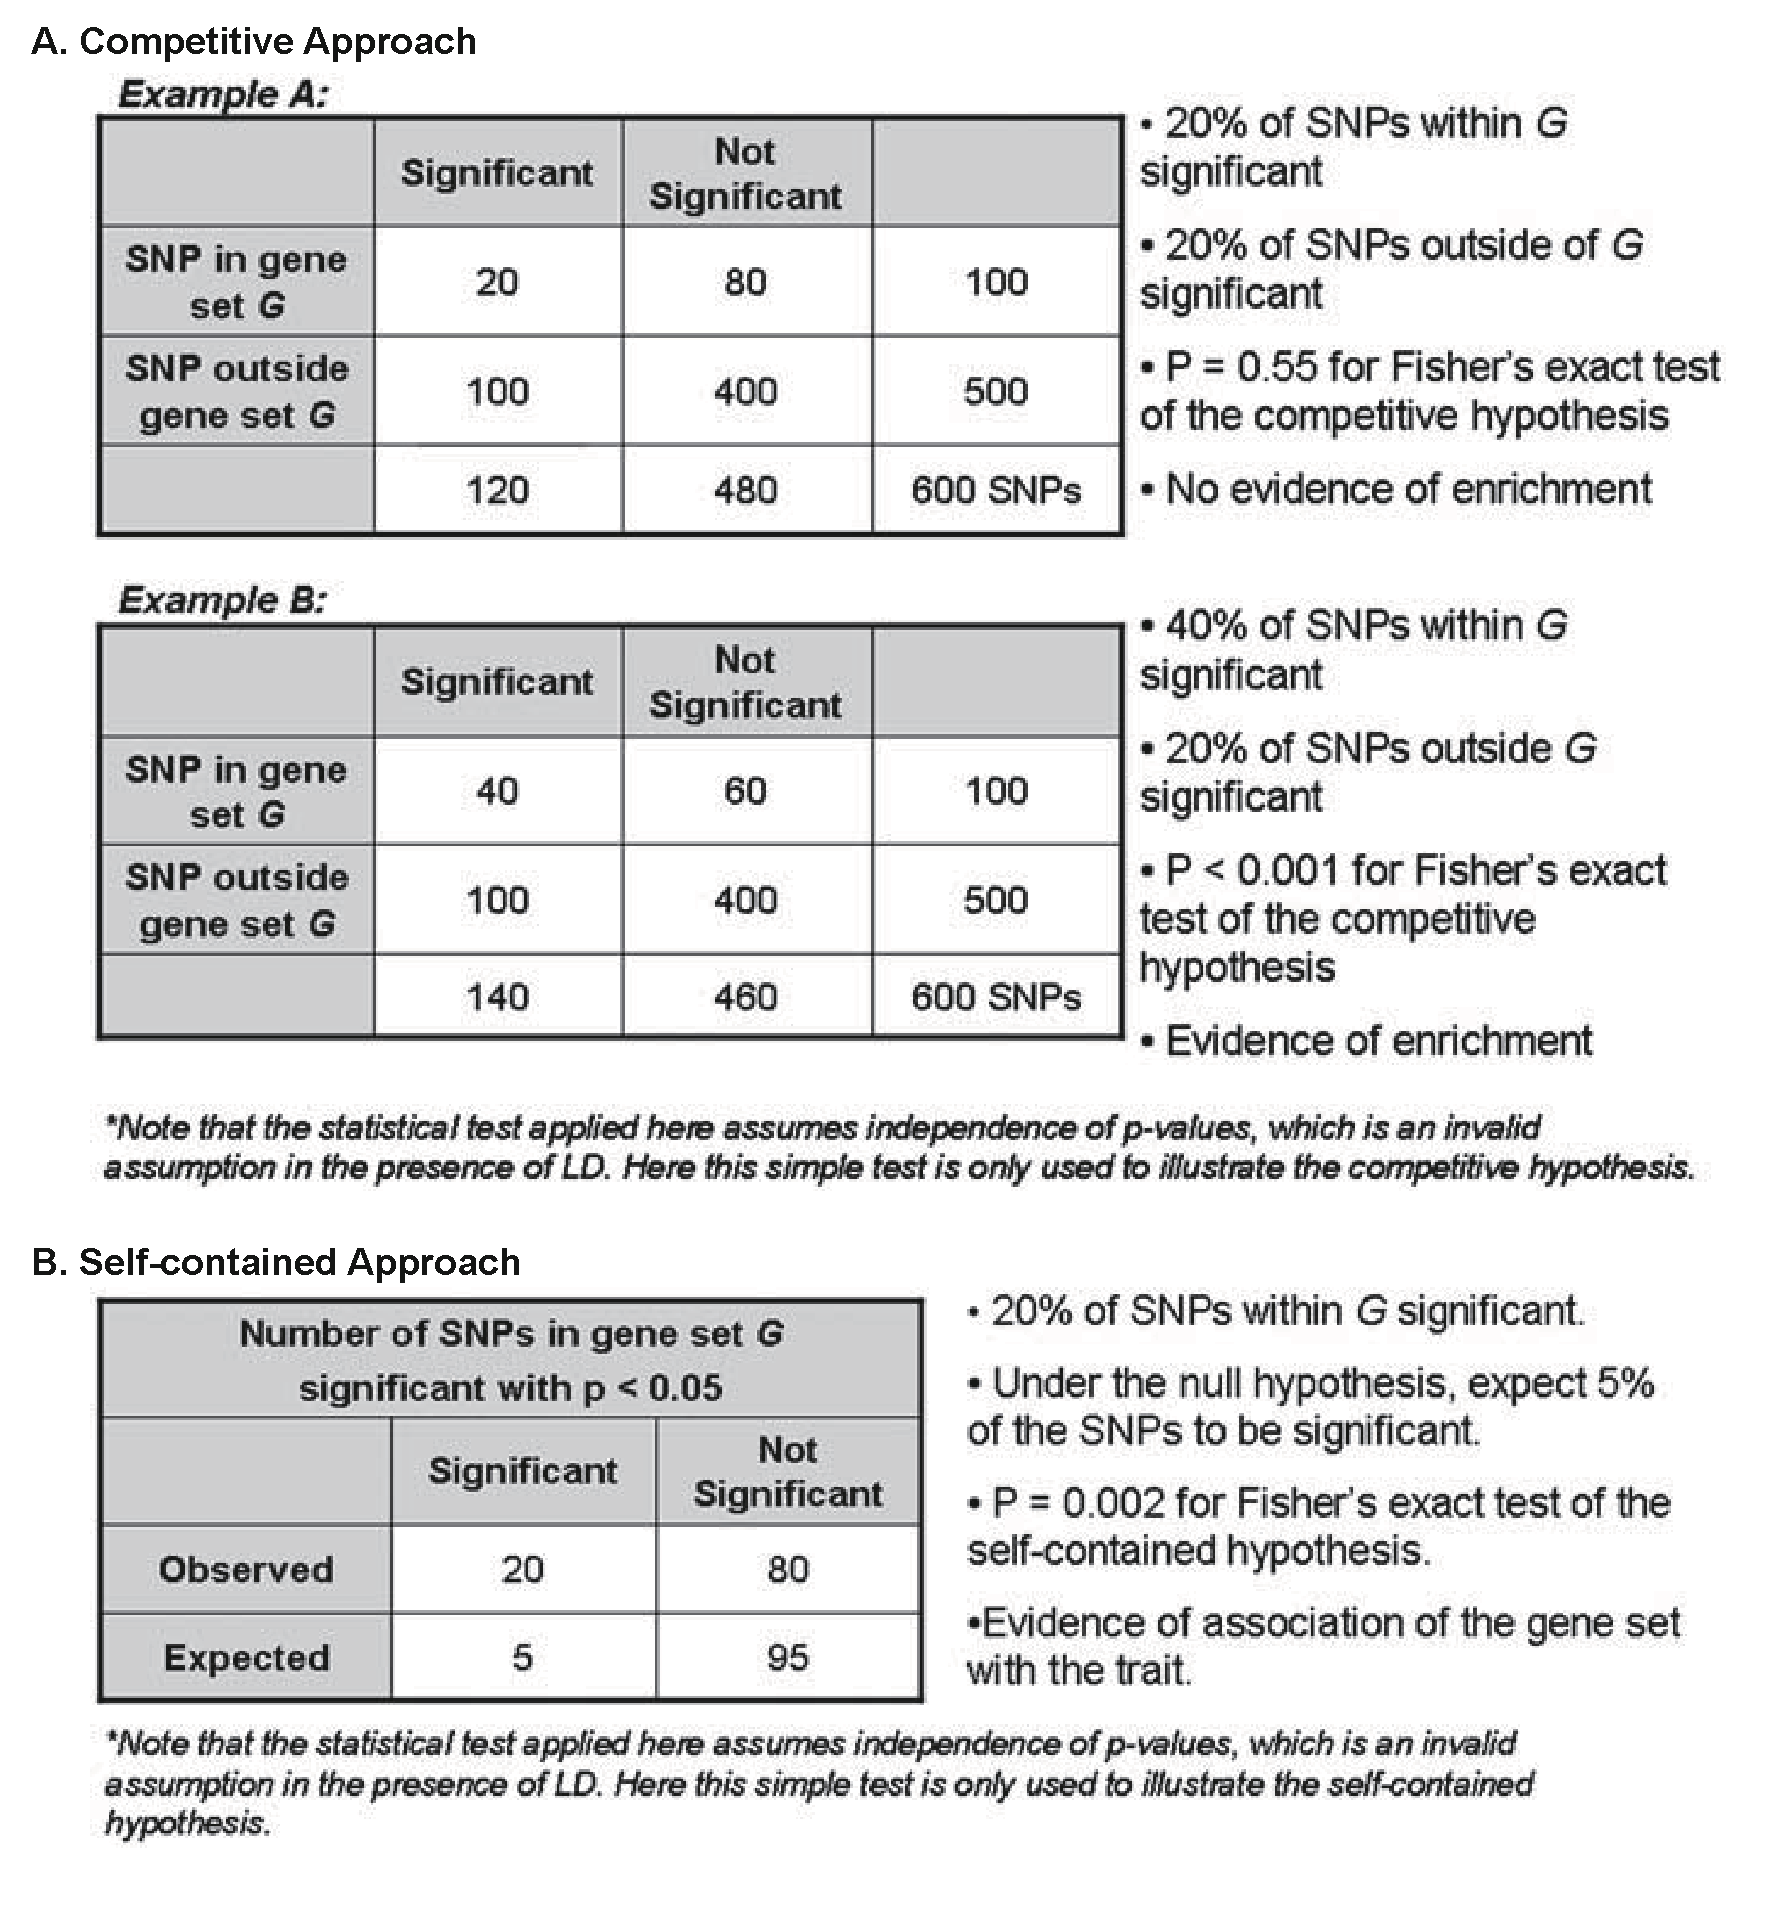
\includegraphics[scale=0.5]{CompetitiveVsConstrained_illustration_example}

\caption{ \textbf{Examples of competitive approach and self-contained approach based testings using Fisher's exact test as a demo} (A). Example of competitive approach; (b). Example of self-contained approach. Figure is adopted from Fridley et al 2010 \cite{Fridley2011}. \label{fig: CompetitiveVsConstrained}}
\end{figure}

Self-contained approach has a few edges over the competitive approach. One limitation of competitive approach is they cannot be applied to studies of candidate gene-sets for
which only SNPs in the candidate gene-sets have been genotyped but not in complemented ones. The reason is straightforward: competitive approach requires a comparison between many different pathways. On the other hand, self-contained approach requires only genotypes from a collection of candidate genes, which in turn enables the genome-wide studies, candidate gene studies, pathway studies or specific disease gene group studies. Specific disease gene group studies are very popular, examples include the cardiovascular diseases, the metabolic traits and the autoimmune diseases. These studies usually came with the disease-specific genotyping platform support, e.g. ImmunoChip \cite{Cortes2011}, metabochip \cite{Voight2012} and CVD35/cardiovascular-IBC-array \cite{Cheng1999,Keating2008}. Self-contained method has also been reported to be more powerful than competitive methods \cite{Goeman2007}. This follows immediately from the fact that the self-contained null hypothesis is more restrictive than the competitive null hypothesis, as noted before. As a result, a self-contained test will almost always reject the null hypothesis for more gene-sets than a competitive null. Nevertheless, some drawbacks of the self-contained approach have been reported, such as the genomic inflation of test statistics is often observed or not adequately adjusted. It finally leads to an inflated type I error \cite{wang2007pathway,Goeman2007,Fridley2010}; the "single-gene-pitfall", which means when a gene-set/pathway contains only one single gene (rarely happen), the self-contained test will generalize the single gene testing to be equivalent to the gene set testing, in the sense that the two procedures are completely equivalent for singleton gene sets. On the contrary, competitive approach treats the two procedures quite differently \cite{Goeman2007}. 

Additionally, based on input data type, the tests can be broadly classified into two categories: those require raw genotypes and those require a list of SNP p-values. The first approach, 'raw genotype approach', requires raw SNP genotypes as input to derive gene-level and pathway-level test statistics; whereas the second approach, 'p-value enrichment approach', requires a list of pre-calculated SNP p-values to determine whether a specific group of p-values for SNPs (or genes) is enriched for associated signals. The 'p-value enrichment approach' only requires pre-computed SNP pvalues and it greatly saves the labor in coordinating data analysis and data sharing, however, the 'raw genotype approach' provides more flexible solutions such as multi-marker tests which requires individual genotype data to derive gene-level test statistics (some of these methods pool all SNPs in a pathway together without calculating test statistics for pathway gene members). Another example is those methods based on single-marker p-values but require raw genotype data to execute phenotype permutation based test. In this way, those methods can come up with a more unbiased pathway enrichment score. The 'raw genotype approach' is also more unbiased, such as it can adjust for gene length, the distance threshold to assign SNPs to nearby genes and the way to summarize gene-level test statistics. The graphic demo of method categorization is shown in Figure \ref{fig: pathwayTests}.

\begin{figure}[H]
\centering
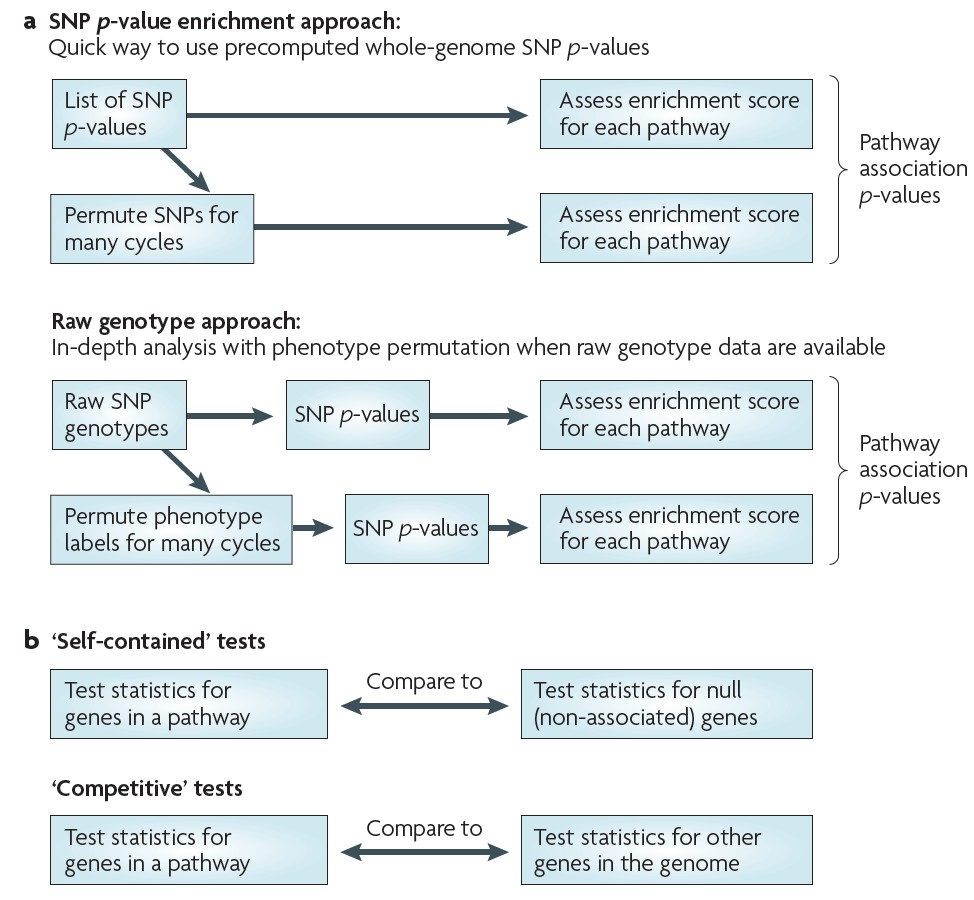
\includegraphics[scale=0.5]{pathwayTests_definition}

\caption{ \textbf{Types of pathway association tests in GWAS.} (a). Categorization based on data input type; (b). Categorization based on hypothesis testing. Figure is adopted from Wang et al 2010 \cite{Wang2010}. \label{fig: pathwayTests}}
\end{figure}

\textbf{Existing pathway based association testing methods}\\
There are several popular existed methods in pathway association testing.  The earliest method is gene-set enrichment analysis (GSEA) algorithm, a method adapted for pathway-based analysis of GWA data, which calculated a weighted Kolmogorov-Smirnov-like running-sum statistics and used permutation-based procedure to come up with statistical significance \cite{wang2007pathway}. The GSEA-SNP, a modification of Wang et al's GSEA \cite{wang2007pathway}, used max-test and all SNPs in a gene \cite{Holden2008}. The i-GSEA4GWAS, first permuted SNP labels, then assigned SNPs to genes, finally calculated the modified GSEA enrichment score\cite{Zhang2010a}. The Gene Set Analysis (GSA-SNP), executed the gene-level test based on the SNP with minimum P-value (or second best), followed by gene-set-level test using either a Z-test, maxmean test, or GSEA \cite{Nam2010}. The Gene Set-based Analysis of Polymorphisms (GeSBAP), first calculated enrichment score using ranked gene list, then assigned the best SNP p-value to a gene, finally used Fisher's exact test for the gene-set association \cite{Medina2009}. A modification of Fisher’s method for combing SNP P-values for gene-level or gene-set-level association \cite{DelaCruz2010}. The gene set ridge regression in association studies (GRASS), executed lasso regression (L1-norm) of eigenSNPs within each gene to achieve variable selection, while performing ridge regression (L2-norm) of eigenSNPs at the gene-set-level to achieve gene effect (e.g. disease risk odds) estimates shrinkage simultaneously \cite{Chen2010}. PLINK, a very famous software in GWA data analysis, provided an option to execute gene-set-level association analysis \cite{Purcell2007}. The association list go annotator (ALIGATOR), a 'p-value enrichment approach' requiring only pre-computed SNP p-values, used Fisher's exact test on SNP with minimum p-value for the gene-level association. It can correct for linkage disequilibrium (LD) between SNPs, various gene size, and multiple testing of nonindependent pathways \cite{Holmans2009}. The SNP ratio test (SRT), tested the ratio of significant SNPs in a pathway and compute the empirical p-value based on permutation \cite{ODushlaine2009}. The supervised principal component analysis, used the Gumbel extreme value mixture distribution as test statistic distribution and standardized for pathway size using simulation procedure \cite{Chen2010a}. Prioritizing Risk Pathways fusing SNPs and pathways (PRP), executed the gene-level association test based on max risk statistic, followed by mean risk approach to get gene-set-level risk statistic, then weighted this statistic by specific pathway degree (i.e. total edges in a pathway) and standardized to zero dimension \cite{Chen2009}. Three statistics combined a set of dependent p-values of SNPs into an overall significance level for a gene, and then combined a set of dependent p-values of genes into an overall significance level for a pathway. The three statistics, which take into account the LD among SNPs or correlation among genes in the specific pathway, are linear combination test (LCT) asymptotically following normal distribution under null hypothesis; Quadratic test (QT) asymptotically following central Chi-square distribution under null hypothesis; and decorrelateion test (DT) combineing decorrelated individual statistics by Fisher's combination test and asymptotically following a central Chi-square distribution under null hypothesis \cite{Luo2010}. Four combination methods of combing a list of SNP p-values or gene-level pvalues with the assumption that individual markers/genes are independent: Fisher's, Sidak's, Simes' and the FDR method \cite{peng2009gene}. The Gene-loci Set Analysis (GLOSSI), first used the Cochran-Armitage trend test at single-marker level test assuming an additive SNP effect, then used Fisher's combination test to combine individual p-values of markers, finally corrected test statistics by Brown's approximation to better control the type I error \cite{Chai2009}. An adaptive rank truncated product (ARTP) statistic, combined permutation-based marker-level p-value to derive gene-level significance level and/or combine gene-level p-values to derive pathway-level significance level \cite{Yu2009}. Detailed reviews about such pathway-level association tests can be found in \cite{tintle2011inflated,Wang2010,Fridley2011}. 

\section{Public Health Significance}\label{sec:PHsig}
The majority of human diseases are complex diseases, e.g. cardiovascular disease, type 2 diabetes, Alzheimer's disease and autoimmune disease. These diseases have high incidence rate in the US and worldwide \cite{Craig2008,Cardon2001,Hirschhorn2005}. The development of complex diseases involves genetic factors, environmental factors, behavior factors, and the interactions among them. In Public Health research, identification of the casual factors and the heritability of complex disease has always been a frontier topic. Researchers look for the genetic factors at first, then they conduct secondary wave analyses like gene-gene and gene-environment interaction analyses.  The GWASs have already identified more than 1000 genetic loci associated with many human disease and traits \cite{Hindorff2009}. However, further studies validated some of these loci are actually false positives. Researchers thus proposed a few solutions, such as more powerful tests, meta analysis and wet lab experiment validation, to remedy this problem \cite{Wang2005,Hirschhorn2005,McCarthy2008,Hindorff2009,Cantor2010}. 

The advent of Next-Generation Sequencing techniques have brought human genetics to a new era \cite{Ansorge2009,Metzker2009,Mardis2008,Shendure2008}, and have the potential to explain some of the missing heritability via disease/trait-associated rare variants \cite{Eichler2010}. Researchers have delivered tremendous efforts in developing powerful association tests either for common variants or rare variants, in gene-based and/or pathway-based manner as aforementioned. These tests are were majorly designed for cross-sectional data analysis, which utilizes less information and is thus less powerful then longitudinal data analysis. Although some of these tests have the flexible framework underpinned to enable extending themselves to accommodate the longitudinal data scenario, the development is not yet done or still undergoing (unpublished). As the association pattern between variants and disease/trait is subtle and unpredictable, more and more novel association tests focused on providing user an "data-adaptive" style tests. The so-called "data-adaptive" test can maintain the most power for various real world data sets. Combining all these thoughts, in my dissertation, the statistical method development will provide researchers a more powerful and robust data adaptive association test for either CVs or RVs under longitudinal data settings. Both gene-based and pathway-based test strategies will be implemented. Besides, an R package or independent Linux command-line based software implementing the methods will be released shortly after the methodology development, which will greatly facilitate community to use the new methods on real data. In conclusion, my dissertation work will provide useful methods/tools to identify the underlying genetic factors and explain the heritability of human complex disease. In the long run, it will contribute to the prevention, diagnosis and cure of complex diseases.
% \newpage
%%%%%%%%%%%%%%%%%%%%%%%%%%%%%%%%%%%%%%%%%%%%%%%%%%%%%%%%%%%%
\section{Specific Aims and Hypotheses}\label{sec:aims}
%%%%%%%%%%%%%%%%%%%%%%%%%%%%%%%%%%%%%%%%%%%%%%%%%%%%%%%%%%%%
As reviewed herein before, current association test methods were mainly designed for cross-sectional data analysis. However, many GWA data did have longitudinal measurements, e.g. the Atherosclerosis Risk in Communities (ARIC) study \cite{Chambless1997} has multiple follow-up measurements across years. Tests fully utilizing the information across time points tend to achieve a greater power and identify more disease-related loci \cite{Furlotte2012,Xu2014}. As both the common variants and rare variants are important in identifying the disease attributing factors, a well-rounded association test should have the flexibility to work with either of them. The test should also maintain a relatively high power in almost all scenarios of the real world data sets. In real world, it is hard to predict which specific method has the greatest power and which methods suffer from large power loss over a specific data set. To meet these urgent needs, a powerful data-adaptive SNP-set-based association test is proposed for longitudinal data analysis, workable on either CVs or RVs. The detailed aims are:
%%%%%%%%%%%%%%
%%%%%%%%%%%%%%
\subsection{Aim One: Data-adaptive association tests for longitudinal data analysis within GEE framework}
%\begin{enumerate}
%\item \textbf{Aim One}
Develop the robust data-adaptive association test for longitudinal data analysis within the Generalized Estimating Equation framework, which has relatively high power in most data scenarios and avoid drastic power loss in any single data scenario, as compared to current available methods. This is the first data-adaptive association test method for longitudinal data as to my knowledge.
%%%%%%%%%%%%%
\subsubsection{1(a): A data-adaptive association test for longitudinal data analysis within GEE framework}
%\begin{enumerate}
%\item[(1a)]
Develop the data-adaptive longitudinal association test within GEE framework workable for common variants, which will be done in either sliding-window based or gene-based manner for real GWAS data. Since CVs are usually coming from traditional SNP genotyping platform (e.g. selection of tagging SNPs), the SNPs are almost evenly distributed on the whole chromosome. To include, say a constant number of 40 SNPs, the regions covering the 40 SNPs on a chromosome are by large of the same physical length (e.g. 1kb), which makes the slide-window based manner reasonable to detect signals from a specific chromosome region. Gene-based manner has been extensively discussed in section \ref{sec:background}. Since missing data scenario is usually the case in longitudinal data analysis, e.g. an individual has three out of four total measurements, the developed algorithm is expected to utilize the partial information fully instead of deleting the whole subject, and still provides consistent coefficients estimates as long as the data missing follows the Missing At Complete Random (MACR) rule \cite{rubin1976inference,Xu2014}.

[To Dr. Morrison's concern: Add the paragraph of introducing the simulation and analysis of the ARIC data in Aim section]\\
We will test the proposed novel method's performance using simulated data. Specifically, we will simulate genetics data and longitudinal trait data mimicking real data scenario, e.g. genetics data will allow LD structure among SNPs and longitudinal trait will have flexible control over the between-subject variance, the within-subject variance, the number of measurements and the correlation structure among measurements. We will benchmark our new test against several existing methods, such as Sum test, UminP test and Score test. Specifically, we will test whether the type I error could be controlled at the nominal level (neither inflated nor conservative), and compare the empirical power under different simulation scenarios.
%%%%%%%%%%%%%%%%%%%
\subsubsection{1(b): Longitudinal aSPU family tests on Rare Variants}
%\item[(1b)]
Extend the data-adaptive longitudinal association test within GEE framework to work for rare variants in a gene-based manner. Since RVs has much lower MAFs than CVs, assumptions such like coefficient estimator follows an asymptotic normal distribution may not hold any more. Procedures like permutation or parametric bootstrap designed for the longitudinal data settings should be adopted to provide a more accurate association significance level.

[To Dr. Morrison's concern: Add the paragraph of introducing the simulation and analysis of the ARIC data in Aim section]\\
We will test, on simulation data (genetic and longitudinal trait), the effect after adopting permutation or parametric bootstrap strategy. We expect to see such procedures can provide a better control of type I error and a more unbiased estimate of the real power.

[To Dr. Morrison's concern: special ways that lipids must be treated when analyzing the ARIC data]\\
We will apply the novel method to ARIC cohort data as mentioned in section \ref{sec:data}. Since the ARIC cohort data currently have \textbf{five} follow-ups till now, they are perfect data for my dissertation research on longitudinal data-adaptive association test. We propose to use four closely cardiovascular-disease-related traits measured in ARIC cohort data as our response variables, which are total cholesterol (tch), High-density lipoprotein (HDL), Low-density lipoprotein (LDL) and triglycerides (trgs). We will fit each trait separately by our proposed method. We will \textbf{take cautions before using these lipid traits} such as accounting for lipid-lowering therapy in TC and LDL traits, and natural log transformation on the trgs trait according to the procedures described in \cite{Peloso2014}. We will use genotype data either from traditional microarray genotyping platform for CVs or ExomeChip platform for RVs. We expect to validate known genetic loci as reported in literature \cite{Teslovich2010,Lange2014,Peloso2014,Consortium2013,Maxwell2013} as well as identifying potential novel genetic loci associated with any of these traits. We will exclusively use Caucasian samples in this study. To adjust for necessary covariates, we will include but not limited to subject's demographic information such as age, gender and BMI. The application of the new methods on ARIC cohort data, on one hand, will help evaluate the performance of proposed methods; on the other hand, it has the potential to identify more genetic loci contributed to atherosclerosis risk.
%\end{enumerate}
%%%%%%%%%%%%%%%%
%%%%%%%%%%%%%%%%
\subsection{Aim Two: Pathway-based longitudinal aSPU family tests: Path-aSPU}
%\item \textbf{Aim Two}
Extend the data-adaptive longitudinal association test within GEE framework to work for common variants or rare variants in a gene-set/pathway-based manner, e.g., pathway-based association test. Currently, there are no statistical models designed for pathway-based association test in longitudinal data settings, not to mention the data-adaptive property.

[To Dr. Morrison's concern: Add the paragraph of introducing the simulation and analysis of the ARIC data in Aim section]\\
We will simulate the gene pathway including multiple genes, and each gene contains multiple SNVs. We will test our Path-aSPU's performance in controlling type I error and maintaining a higher power under different simulation scenarios. We will compare Path-aSPU to a few existing tests such like SSU, Score, Sum, and UminP test. Although other existing tests like GRASS \cite{Chen2010} and ALIGATOR \cite{Holmans2009} are very famous pathway-based association tests, they were designed for cross-sectional data analysis, and thus unavailable to compare with.

With regard to data application, we will define the gene pathway by public pathway resources like KEGG \cite{Ogata1999} and BioCarta \cite{Nishimura2001}. We will apply Path-aSPU on ARIC data to find significant association between a specific pathway and a specific longitudinal trait.
%%%%%%%%%%%%%%%%
%%%%%%%%%%%%%%%%
\subsection{Aim Three: Package/software development}
%\item \textbf{Aim Three}
Provide an R package or a Linux command-line based software program to enable convenient implementation of above methods. The package/software will be released to public (e.g. CRAN) eventually.
%\end{enumerate}

\newpage
%%%%%%%%%%%%%%%%%%%%%%%%%%%%%%%%%%%%%%%%%%%%%%%%%%%%%%%%%%%%
\section{Real Data Introduction}\label{sec:data}
%%%%%%%%%%%%%%%%%%%%%%%%%%%%%%%%%%%%%%%%%%%%%%%%%%%%%%%%%%%%
[To Dr. Morrison's concern: revise real data introduction, e.g. remove unnecessary figure and add description of fifth follow-up measurement]
%Real data used in my dissertation will be obtained from
%the Atherosclerosis Risk in Communities (ARIC) Study (https://www2.cscc.unc.edu/aric/). The Atherosclerosis Risk in Communities Study (ARIC), sponsored by the National Heart, Lung, and Blood Institute (NHLBI) is a prospective epidemiological study conducted in four U.S. communities.  ARIC is designed to investigate the causes of atherosclerosis and its clinical outcomes, and variation in cardiovascular risk factors, medical care, and disease by race, gender, location, and date. To date, the ARIC project has published over 800 articles in peer-reviewed journals. ARIC includes two parts: the Cohort Component and the Community Surveillance Component. %The ARIC study is a longitudinal cohort study designed to ascertain the etiology and predictors of cardiovascular disease (CVD). The ARIC study enrolled 15,792 middle-aged adults from four U.S. communities (Forsyth County, NC; Jackson, MS; suburbs of Minneapolis, MN; and Washington County, MD) between 1987–89 and followed by four completed visits with each approximately three years apart, in 1987–89, 1990–92, 1993–95, and 1996–98. In general, each visit included interviews and a physical examination. A detailed description of the ARIC study design and methods was published elsewhere [39]. 
%
%The Cohort Component of the ARIC study, which will be applied to our new methods, began in 1987, and each of the four ARIC field centers (Washington County, MD; Forsyth County, NC; Jackson, MS; and Minneapolis, MN) randomly selected and recruited a cohort sample of approximately 4,000 individuals aged 45-64 from a defined population in their community. A total of 15,792 participants received an extensive examination, including medical, social, and demographic data.  These participants were re-examined every three years with the first screen (baseline) occurring in 1987-89, the second in 1990-92, the third in 1993-95, and the fourth exam was in 1996-98. The fifth screen is farther apart from the previous screens and was finished during 2011-2013. A detailed description of the ARIC study design and methods was published elsewhere \cite{Investigators1989}.
%%In 2009, the NHLBI funded a fifth exam, which is currently being conducted.
%
%%In the Community Surveillance Component, the four communities are investigated to determine the long term trends in hospitalized myocardial infarction (MI) and coronary heart disease (CHD) deaths in approximately 470,000 men and women aged 35-84 years.\\
Real data used in my dissertation will be obtained from the Atherosclerosis Risk in Communities (ARIC) Study (https://www2.cscc.unc.edu/aric/). The Atherosclerosis Risk in Communities Study (ARIC), sponsored by the National Heart, Lung, and Blood Institute (NHLBI), is a prospective epidemiological study conducted in four U.S. communities. ARIC is designed to investigate the causes of atherosclerosis and its clinical outcomes, the variation in cardiovascular risk factors, medical care, and disease by race, gender, location, and time. To date, the ARIC project has published over 800 articles in peer-reviewed journals. ARIC data include two parts: the Cohort Component and the Community Surveillance Component.

The Cohort Component of the ARIC study, on which we will apply our proposed methods, began in 1987. Each of the four ARIC field centers (Washington County, MD; Forsyth County, NC; Jackson, MS; and Minneapolis, MN) randomly selected and recruited a cohort sample of approximately 4,000 individuals aged 45-64 from a defined population in their community. A total of 15,792 participants received an extensive examination, including medical, social, and demographic data. These participants were re-examined every three years with the first screen (baseline) occurring in 1987-89, the second in 1990-92, the third in 1993-95, and the fourth exam was in 1996-98. The fifth screen is farther apart from the previous screens and was finished during 2011-2013. A detailed description of the ARIC study design and methods was published elsewhere \cite{Investigators1989}.

%%%%%%%%%%
%%%%%%
%%%
%%
% Dr. Morrison pointed out this figure should be removed as it is not appropriate.
%To help the audience to gain a fast and general understanding of the ARIC data two components, I borrowed a flowchart from the ARIC website here as in Figure \ref{fig: ARICcomponents}
%\begin{figure}[H]
%\centering
%\includegraphics[width=1\textwidth]{{{ARICcomponents}}}
%\caption{ARIC Cohort and Community Surveillance Components. Figure adopted from the ARIC website}
%\label{fig: ARICcomponents}
%\end{figure}


%\textbf{The objectives of the ARIC Study}
%\begin{itemize}
%\item \textbf{Examine} the ARIC cohort to characterize heart failure stages in the community, identify genetic and environmental factors leading to ventricular dysfunction and vascular stiffness, and assess longitudinal changes in pulmonary function and identify determinants of its decline.
%
%\item \textbf{Cohort follow-up} for cardiovascular events, including CHD, heart failure, stroke, and atrial fibrillation; and for the study of risk factors related to progression of subclinical to clinical CVD.
%
%\item \textbf{Enhance} the ARIC cohort study with cardiovascular outcomes research to assess quality and outcomes of medical care for heart failure and heart failure risk factors.
%
%\item \textbf{Community surveillance} to monitor long-term trends in hospitalized MI, CHD deaths, and heart failure (inpatient and outpatient).
%
%\item \textbf{Provide} a platform for ancillary studies, training for new investigators, and data sharing.
%\end{itemize} 


%\textbf{The objectives of my dissertation usage of ARIC data}\\
%Since the ARIC cohort data currently has five follow-ups till now, it's a perfect data set for my dissertation research on data-adaptive association test for longitudinal data. We propose to use four closely cardiovascular-disease-related traits measured in ARIC cohort data, which are total cholesterol (tch), High-density lipoprotein (HDL), Low-density lipoprotein (LDL) and triglycerides (trgs), as our response variables (will fit each one separately by our proposed model). We hope to validate known genetic loci as reported in literatures \cite{Teslovich2010,Lange2014,Peloso2014,Consortium2013,Maxwell2013} as well as identifying potential novel genetic loci associated with any of these traits. We will exclusively use Caucasian samples. For the covariates, we will include but not limited to subject's demographic information such as age, gender and BMI. The application of the new methods on ARIC cohort data will on one hand help evaluate the performance of proposed methods, and on the other hand will have chance to identify more genetic loci contributed to atherosclerosis risk.

A demographic introduction of the ARIC cohort data is shown in Figure \ref{fig: ARIC_CohortCharacteristics}
\begin{figure}[H]
\centering
\includegraphics[scale=0.75]{{{ARIC_CohortCharacteristics}}}
\caption{ARIC Cohort Characteristics by Gender or Race. Table adopted from the ARIC website }
\label{fig: ARIC_CohortCharacteristics}
\end{figure}

%%%%%%%%%%%%%%%%%%
\textbf{Human Subjects}\\
The dissertation study will focus on statistical method development. I will use ARIC cohort component data for method demonstration purpose only. The ARIC data can be freely requested at (https://www2.cscc.unc.edu/aric/distribution-agreements). I will use the phenotype (several traits aforementioned) and genotype (SNP array or ExomeChip) data, which are all de-identified. The IRB approval of the use of ARIC data in my dissertation research has been obtained by my dissertation advisor, Dr. Peng Wei, from UTHealth IRB (HSC-SPH-13-0492) for the NIH funded project "Association analysis of rare variants with sequencing data".


%%%%%%%%%%%%%%%%%%%%%%%%%%%%%%%%%%%%%%%%%%%%%%%%%%%%%%%%%%%%
\section{Methods}\label{sec:method}
%%%%%%%%%%%%%%%%%%%%%%%%%%%%%%%%%%%%%%%%%%%%%%%%%%%%%%%%%%%%
%To get the adjusted P-value for MinP, one generally needs a two-level permutation procedure
%[Hoh, et al. 2001; Westfall and Young 1993] with the inner level for estimating and the
%outer level for the adjustment needed to account for multiple testing over different truncation
%Yu et al. Page 3
%Genet Epidemiol. Author manuscript; available in PMC 2009 December 8.
%NIH-PA Author Manuscript NIH-PA Author Manuscript NIH-PA Author Manuscript
%points. This type of permutation procedure, however, can become computationally infeasible
%if the number of tests L is relatively large. We propose to use a single layer of permutation for
%determining the significance level of the ARTP statistic by borrowing techniques originally
%introduced for gene-expression data analysis [Ge, et al. 2003]. We first obtain P-values for
%Ge et al. [Ge, et al. 2003] to avoid the computationally intensive multilevel
%permutation procedure.
%%%%%%%%%%%%%%%%%%%%%%%%%%%%%%%%%%%%%%%%
\subsection{Aim One (1a): A data-adaptive association test for longitudinal data analysis within GEE framework}\label{sec:subsec1}
%%%%%%%%%%%%%%%%%%%%%%%%%%%%%%%%%%%%%%%%

%%%%%%%%%%%%%%%%%%%%%%%%%%%%%%%%%%%%%%%%
\subsubsection{Statistical Modeling}\label{sec:subsub1-1}
%%%%%%%%%%%%%%%%%%%%%%%%%%%%%%%%%%%%%%%%%
Suppose for each subject $i = 1,\ldots,n$, we have $k$ total longitudinal measurements $y_i = (y_{i1}, y_{i2}, \ldots, y_{ik})'$ with $y_{im}$ as a element, $p$ SNPs of interest as a row vector $x_i = (x_{i1}, x_{i2}, \ldots, x_{ip})$ with $x_{ij}$ coded as 0,1 or 2 for the count of the minor allele for SNP $j = 1, \ldots, p$, and $z_i = (z_{i1}, z_{i2}, \ldots, z_{iq})$ is a row vector for $q$ variates. We assume common effect sizes (a.k.a., time-averaged group effect) of the SNPs and covariates on the longitudinal phenotype/trait measurements. Thus, we construct the design matrix for the SNPs and covariates as:
$$
  X_i = \begin{pmatrix}
          x_{i}\\
          x_{i}\\
          \vdots\\
          x_{i}
          \end{pmatrix} 
  , 
  Z_{i}=\begin{pmatrix}1 & z_{i}\\
          1 & z_{i}\\
          \vdots & \vdots\\
          1 & z_{i}
          \end{pmatrix}
$$
where $x_i$ and $z_i$ are row vectors of length p and q respectively. $X_i$ is a $k \times p$ matrix, and $Z_{i}$ is a $k \times (q+1)$ matrix. Denote the regression coefficient $\beta = (\beta_1, \beta_2, \ldots, \beta_p)'$ and $\varphi = (\varphi_1, \varphi_2, \ldots, \varphi_{q+1})'$ for $X_i$ and $Z_i$ respectively. The marginal mean of each measurement, $E(y_{im}|x_i,z_i) = \mu_{im}$ where $m = 1,2, \ldots, k$ for $k$ total measurements, or the vectorized format of all measurements, $E(y_{i}|x_i,z_i) = \mu_{i}$, relates to the SNPs and covariates through a generalized linear model (GLM):
$$
g(\mu_i) = \eta_i = Z_i \varphi + X_i \beta = H_i \theta
$$
\noindent with $H_i = (Z_i, X_i), \theta = (\varphi', \beta')'$ and $g(.)$ as a suitable link function. For continuous outcome, an identity link is usually used.

The consistent and asymptotically Normal estimates of $\beta$ and $\varphi$ can be obtained by solving the GEE \cite{liang1986longitudinal}: 

\begin{align*}
U(\varphi,\beta) & =\sum_{i=}^{n}U_{i}(\varphi,\beta)=\sum_{i=1}^{n}(\frac{\partial\mu_{i}}{\partial\theta'})'V_i^{-1}(Y_{i}-\mu_{i})=0,\\
\textrm{with}\\
\frac{\partial\mu_{i}}{\partial\theta'} & =\frac{\partial g^{-1}(H_{i}\theta)}{\partial\theta'}, V_i = \phi A_{i}^{\frac{1}{2}}R_{w}A_{i}^{\frac{1}{2}},\\
\textrm{and}\\
A_{i} &= 
\begin{bmatrix}
 v(\mu_{i1}) & 0 & \cdots & 0\\
 0 & v(\mu_{i2}) & 0 & 0\\
 \vdots & 0 & \ddots & \vdots\\
 0 & 0 & \cdots & v(\mu_{ik})
\end{bmatrix}
\end{align*}

$\phi$ in $V_i$ is the dispersion parameter in GEE and is usually treated as nuisance parameter. $v(\mu_{im}) = \phi \textrm{Var}(y_{im} | x_i, z_i) $. $R_w(\alpha)$ is a working correlation matrix depending on some unknown parameter $\alpha$. For convenience, a working independence model
with $R_w = I$ is often used. With a canonical link function and a working independence model, we have a closed form of the U vector with two parts corresponding to SNPs and covariates, and its covariance estimator:
\begin{align}
U & =\left(U_{.1}',U_{.2}'\right)'=\sum_{i}\left(Z_{i},X_{i}\right)'(Y_{i}-\mu_{i})\nonumber \\
% \vspace{-2em}
\widetilde{\Sigma} & = \widehat{\textrm{Cov} }(U) = \sum_{i}\left(Z_{i},X_{i}\right)'\widehat{\textrm{var}(Y_{i})}\left(Z_{i},X_{i}\right)=\sum_{i}\left(Z_{i},X_{i}\right)'(Y_{i}-\hat{\mu_{i}})(Y_{i}-\hat{\mu_{i}})'\left(Z_{i},X_{i}\right)=\begin{pmatrix}V_{11} & V_{12} \\
V_{21} & V_{22}
\end{pmatrix}
\label{eq:1}
% \end{alignat}
\end{align}
where $\hat \mu_i$ is an estimator of $\mu_i$, $\widetilde{\Sigma}$ is an estimate of the covariance of score (U) vector. $\widetilde{\Sigma}$ is partitioned with the dimensions according to the score vector component $U_{.1}$ and $U_{.2}$ for $\varphi$ and $\beta$ respectively.

\textit{Quantitative traits}\\
\indent We use the identity link, i.e. $g(\mu_{im}) = \mu_{im}$ and $v(\mu_{im}) = \phi \times 1 = \phi$. Then we have:
\begin{align}
U & = \sum_{i}\left(Z_{i},X_{i}\right)' R_w^{-1} (Y_{i}-\mu_{i}) \nonumber\\
\widetilde{\Sigma} & = \sum_{i}\left(Z_{i},X_{i}\right)' R_w^{-1} (Y_{i}-\hat{\mu_{i}})(Y_{i}-\hat{\mu_{i}})' R_w^{-1} \left(Z_{i},X_{i}\right)
\label{eq:2}
\end{align}

if the assumption of a common covariance matrices across $Y_i$ for $i$ is valid, e.g. for quantitative continuous traits study \cite{pan2001robust}, we can adopt a more efficient covariance estimator:
\begin{align*}
\widetilde{\Sigma} & = \sum_{i=1}^n \left(Z_{i},X_{i}\right)'\widehat{\textrm{var}(Y_{i})}\left(Z_{i},X_{i}\right)
 = \sum_{i=1}^n \left(Z_{i},X_{i}\right)'\left(\sum_{i=1}^n \frac{(Y_{i}-\hat{\mu_{i}})(Y_{i}-\hat{\mu_{i}})'}{n}\right)\left(Z_{i},X_{i}\right) = 
\begin{pmatrix}
V_{11} & V_{12}\\
 V_{21} & V_{22}
\end{pmatrix}
\end{align*}
which is used by default for its better finite-sample performance \cite{pan2001robust}.

In my dissertation, I will \textbf{focus on} the case with quantitative traits, since they are most typical traits used as response variable in longitudinal data analysis. Nevertheless, I introduce the binary traits strategy as below. In general, the only difference lies in which canonical link we will use, with all other equations/formulas keep the same.

\textit{Binary traits}\\
\indent For binary traits (trait value coded as 0 and 1), we use the logit link function so that $g(\mu_{im}) = log \frac{\mu_{im}}{1 - \mu_{im}}$ and $v(\mu_{im}) = \mu_{im} (1 - \mu_{im})$. Additionally the $(m, l)$th element of $\frac{\partial\mu_{i}}{\partial\theta'}$ is
$
H_{i,ml} \mu_{im} (1- \mu_{im})
$
with $H_{i,ml}$ as the $(m, l)$th element of $H_i$, which is the short notation for $(Z_{i},X_{i})$.\\
Then we have:
\begin{align*}
U & = \sum_{i=1} (\frac{\partial\mu_{i}}{\partial\theta'})' V_i^{-1} (Y_{i}-\mu_{i})\\
& = \sum_{i=1} (\frac{\partial\mu_{i}}{\partial\theta'})' \phi A_{i}^{-\frac{1}{2}} R_{w}^{-1} A_{i}^{-\frac{1}{2}} (Y_{i}-\mu_{i})\\
\end{align*}
and
\begin{align*}
\widetilde{\Sigma} & = \sum_{i}\left(\frac{\partial\mu_{i}}{\partial\theta'}\right)' \phi A_{i}^{-\frac{1}{2}} R_{w}^{-1} A_{i}^{-\frac{1}{2}} (Y_{i}-\hat{\mu_{i}}) (Y_{i}-\hat{\mu_{i}})' \phi A_{i}^{-\frac{1}{2}} R_{w}^{-1} A_{i}^{-\frac{1}{2}} \left( \frac{\partial\mu_{i}}{\partial\theta'} \right)\\
& = 
\begin{pmatrix}
V_{11} & V_{12}\\
 V_{21} & V_{22}
\end{pmatrix}
\end{align*}
%%%%%%%%%%%%%%%%%%%%%%%%%%%%%%%%%%%%%%%%%%%%%%%%%%%%%%%%%%%%%%%%%%%%%%%%%%%%%%%%%%%%%%%%%%%%%%%%%%%%

\textit{Several Current Association Tests}\\
Our goal is to detect whether there is any association between the longitudinal trait and the SNPs via testing on hypothesis $H_{o}:\beta=(\beta_{1},\beta_{2},\ldots,\beta_{p})'=0$. We have under the null hypothesis with $g(Y_i)=Z_i\varphi$ to obtain $\varphi$ and predict $\hat{\mu}=g^{-1}(Z\hat{\varphi})$. We hereby have score vector under the null hypothesis, with a working independence model, is:
$$U(\hat{\varphi},0)=(U_{.1}^{'}, U_{.2}^{'})'=\sum_{i=1}^{n}(U_{i1}^{'},U_{i2}^{'})'$$
where
$$U_{.1}=\sum_{i}Z_{i}'(Y_{i}-\hat{\mu_{i}}), U_{.2}=\sum_{i}X_{i}'(Y_{i}-\hat{\mu_{i}})$$ 
As $U$ asymptotically follows a multivariate normal distribution under $H_{0}$, then the score vector for $\beta$ also has an asymptotic normal distribution:\\
$$
U_{.2}\sim N(0,\Sigma_{.2}),\,\Sigma_{.2}= \widehat{Cov} (U_{.2}) = V_{22} - V_{21} V_{11}^{-1} V_{12}
$$, where $V_{xx}$ are defined in Equation \ref{eq:1}.
\begin{itemize}
\item \textbf{The Wald Test:} The Wald Test known as $T=\hat{\beta'}\text{cov (\ensuremath{\hat{\beta}}) }\hat{\beta}$ is most commonly used, where $\hat{\beta}$ is the estimate of $\beta$ after fitting the full GEE model with $g(\mu_i) = Z_i\varphi + X_i \beta$. Under $H_0$, we have $T \sim \chi_{p}^2$. The Wald test is more time consuming by fitting full model, may fail to converge with many SNPs put on RHS of the regression-like equation to test, and even worse, the type I error tends to inflate in such case \cite{pan2014powerful,zhang2014testing}.
\item \textbf{The Score Test:} $T=U_{.2}^{'}\Sigma_{.2}^{-1}U_{.2}^{-1}$, where $U_{.2}$ and $\Sigma_{.2}$ are discussed above; the statistic is asymptotically equivalent to the Wald test with the same null distribution $T \sim \chi_{p}^2$. Since we only need to fit the null model with covariates, it is computationally easier and less likely to have numerical convergence
problems. More importantly, the score test controls the type I error well \cite{pan2014powerful,zhang2014testing}.
\item \textbf{The UminP Test: }$T=\underset{j}{max}\frac{U_{.2,j}^{2}}{\Sigma_{.2,jj}}$
for $j\in 1,2,\dots,p$, of $j$th SNP effect. The $\Sigma_{.2,jj}$ is the $j$th entry on the diagonal of $\Sigma_{.2}$. With max $T$, we can get minimal p-value accordingly. An asymptotic multivariate normal distribution numerical integration based method provided a fast way to calculate its p-value \cite{Pan2009a,Pan2009}; alternatively, a simulation based method relying on the asymptotic normal distribution of the score vector can be used to calculate its p-value \cite{pan2014powerful,zhang2014testing}. Specifically, we first simulate the score vector $U_{(b)} = ( U_{(b).1}, U_{(b).2},\ldots, U_{(b).p} )'$ from its null distribution  $U_{(b)} \sim N(0, \Sigma_{.2} )$ for $b = 1, 2, \ldots, B$, then calculate a total number of B null statistics: $T^{(b)} = \textrm{max}_{j = 1,\ldots,p} { U^2_{(b).j} \over  \Sigma_{.2,jj} }$, and the p-value is calculated as $\sum_{b=1}^B { I(T^{(b)} \geq T ) + 1  \over B + 1 } $.

With a working independence correlation matrix $R_w = I$, every element $\frac{U_{.2,j}^{2}}{\Sigma_{.2,jj}}$ is equivalent to running the model on each single SNP (e.g. $j$th) one by one and get the Score test statistics. Hence, in this condition, the GEE-UminP test is equivalent to the usual UminP test that combines multiple single-SNP based longitudinal association test statistics.
\end{itemize}

\textit{A new class of tests and a data-adaptive test in longitudinal data settings}\\
Before I introduce the proposed new test method, let me explain the logic in current GEE and Score test based methods.
$$
T_{Sum} = 1' U = \sum_{j=1}^p U_j, \qquad T_{SSU} = U'U = \sum_{j=1}^p U_j^2,
$$
These two tests are called Sum test and SSU test \cite{Pan2009}. The former is closely related to other burden tests such like those in \cite{Morgenthaler2007,Li2008,Madsen2009} If there is a common association either in direction or strength for causal SNVs with no or few non-associated SNVs, then Sum test and the likes will be most powerful; otherwise, the SSU test and its closely relatives, such as kernel machine regression (KMR or SKAT) \cite{Lee2012,Ionita-Laza2013,Oualkacha2013,Lee2012a,Wu2011} and C-alpha test \cite{Neale2011}, will be most powerful. 

Sum test and SSU test are all based on score vector. A more general form of score-based statistic can be generalized as:
$$
T_w = W' U = \sum_{j=1}^p W_j U_j
$$
where $W = (W_1, \ldots, W_p)'$ is a vector of weights for the $p$ SNVs \cite{Lin2011}. Different researchers proposed different weighting schemes to pool the information of all SNVs in a region of interest, such as those used in \cite{Madsen2009,Sul2011,Pan2011,Han2010,Li2008,Zhang2011,Lin2011,Basu2011}. However, all of these weighting schema have used fixed weights, for example, their weights were chosen proportional to the MAF of SNV, proportional to the standard deviation of SNV, proportional to the regression coefficient or proportional to the single SNV p-value. There is no uniformly best weighting scheme as shown in \cite{pan2014powerful,Basu2011,Pan2011}. 

As a complement to SNVs weighted average, SNVs selection is preferred in the case that there are many non-associated SNVs among the group of SNVs to be tested. Such methods include aSum+ and aSSU which are based on Neyman-type tests \cite{Neyman1937}. However, variable selection will also omit those variables with mild to moderate information. In our context, due to extremely low MAF of RVs, even underlying fact is that the individual RV is strongly associated with trait, there is only limited information stored in this single RV. Dumping seemingly non-informative RVs may actually omit the signals within the group of SNVs. Therefore, we expect the model averaging based test will outperform the model selection based test in above settings.

\textbf{The SPU test}\\
Our goal is to specify a whole class of weights which can cover a wide range of association patterns: for any given data with unknown association pattern, we hope at least one member of the whole class of weights can render a powerful test. We reason that, since association information is largely maintained in the score vector itself as comparable to regression coefficient, score vector is not only the basis in GEE and Score test based methods aforementioned, but also may be an informative and simple weight! Specifically, we propose a class of weights 
$$W_j = U_{.2, j} ^ { \gamma - 1} $$
for a series of integer value $\gamma = 1,2,\ldots,\infty$, leading to the sum of powered score ($U$) tests called SPU tests:
$$
T_{ SPU ( \gamma ) } = \sum_{j=1}^p U_{.2, j} ^ { \gamma - 1} U_{.2, j}
$$

When $\gamma = 1$, the SPU(1) test uses $\textbf{1}$ as weight and sums up the information contained in all the SNVs in the region of interest, equivalent to Sum test or burden test; when $\gamma = 2$, the SPU(2) test uses $U$ as weight to itself and is equivalent to SSU test and other variance-component test such as SKAT; when $\gamma$ keeps increasing, the SPU($\gamma$) test puts higher weights on the $j$th SNV with larger $|U_{.2,j}|$, while gradually decreasing the weights of other SNVs with smaller $|U_{.2,j}|$. As the large value of $|U_{.2,j}|$ indicates strong association information stored in SNV $j$ and small value of $|U_{.2,j}|$ indicates weak or none association information stored in SNV $j$, a higher $\gamma$ tends to put more and more weights on those informative SNVs. When $\gamma \rightarrow \infty$ as an extreme situation, where $\infty$ is assumed to be an even number, we have
$$
T_{ SPU(\gamma) } \propto ||U||_{\gamma} = \left( \sum_{j=1}^p |U_{.2, j}| ^ { \gamma } \right) ^ { 1 \over \gamma } \ \rightarrow \ ||U||_{\infty} = \textrm{max}_{j=1} ^ p |U_{.2, j}| \equiv T_{ SPU(\infty) }.
$$ 
which takes only the largest element (in absolute value) of score vector. Apparently, SPU($\infty$) is equivalent to UminP test except the variance of each score component is replaced by 1 as in the denominator part.

By above explanation, we can see SPU($\gamma$) test can connect to a few current test with a simplified framework though. Treating $U^{\gamma - 1}$ as the weight with $\gamma \geq 1$ have at least two advantages:\\ 
First, score vector is as informative as a vector of the estimated regression coefficient while being computationally much simpler and more stable in the case of low frequency SNVs. Specifically, since $U_j$ contains association information about SNV $j$ and $U_j$ under null hypothesis follows $N(0, V)$, a larger component of $|U_j|$ corresponds to strong evidence of association between the $j$th SNV and the trait;

%%%%%
Second, it leads to a simple interpretation and a guidance: as the value of $\gamma$ increases, we up-weight more and more the larger components of the score vector while gradually ignoring the remaining components. Such process smoothly combines the variable weighting and variable selection schema. Besides, an even integer of $\gamma$ automatically eliminates the effect of opposite signs of $U_j$, thus avoid power loss due to opposite direction effects canceling out each other; an odd integer of $\gamma$ might be more appropriate, as in SPU(1), Sum test or other burden tests, when the SNV effects are all in the same direction.

In our experience, SPU($\gamma$) test with a large $\gamma > 8$ usually gave similar results as that of SPU($\infty$) test \cite{pan2014powerful}, thus we will only use $\gamma \in \Gamma = \{1,2,\ldots,8,\infty \} $ for the whole dissertation work. Suppose the sample size is large enough or MAF of SNV is large enough for the asymptotic normal distribution of score vector to hold under null hypothesis, we will use a simulation method to calculate the p-value from each $T_{ SPU(\gamma) }$ \cite{Lin2005,Seaman2005}. Specifically, suppose $T$ is short notation of $T_{ SPU(\gamma) }$ for a specific $\gamma$ and $\hat{\Sigma}_{.2}$ is the covariance matrix of the score vector $U_{.2}$ based on original data (see Equation \ref{eq:1}). We draw B samples of the score vector from its null distribution: $U_{.2}^{ (b) } \sim MVN \left( 0, \hat{\Sigma}_{.2} \right)$, with $b = 1,2,\ldots,B$, and thus obtain a statistics under null hypothesis: $T ^ {(b)} = \sum_{j=1}^p U^{ (b)\gamma }_{.2, j} $. We then can calculate the p-value of $T_{ SPU(\gamma) }$ as $P_{ SPU(\gamma) } = \sum_{b=1}^B { I(T^{(b)} \geq T ^ {obs} ) + 1  \over B + 1 } $. 

\textbf{The aSPU test}\\
Although we have a list of SPU($\gamma$) statistics and p-values, we are not sure which one is the most powerful in a specific data situation. Thus, it will be convenient to have a test which data-adaptively and automatically select/combine the best SPU($\gamma$) test(s). We hereby propose an adaptive SPU (aSPU) test to achieve such purpose. There are a list of combining methods, such as exponential combine \cite{Chen2012}, linear combine, quadratic combine and fisher's combine methods \cite{Luo2010,peng2009gene,Derkach2013}. However, in this dissertation work, we will use minimum-p combining method exclusively with room left for trying other combining methods. As for different $\gamma$, it is difficult to characterize the power curve of an SPU test in real data situation, we will use the p-value of a SPU test to approximate its power; this idea has been prevalent in practice. Accordingly, we will have the aSPU test statistic:
$$
T_{aSPU} = \underset{\gamma\in\Gamma}{ \textrm{min} } P_{ SPU(\gamma) },
$$
where $P_{ SPU(\gamma) }$ is the p-value of a specific SPU($\gamma$) test.

Similarly as the above simulation method to get p-value of $T_{ SPU(\gamma) }$, the \textit{same strategy} can be applied to get the p-value of $T_{aSPU}$ and actually it fully utilizes the previous simulated intermediate result, hereby saves another \textit{unnecessary} simulation work. Specifically, at the SPU test stage we already have the $U_{.2}^{ (b) }$ for $b = 1,2,\ldots,B$. We then calculate the corresponding SPU test statistics $T^{ (b) }_{ SPU(\gamma) }$ and p-value 
$$
P^{ (b) }_{ SPU(\gamma) } =  \sum_{b_1 \neq b}^B { I(T^{ (b_1) }_{ SPU(\gamma) } \geq T^{ (b) }_{ SPU(\gamma) } ) + 1  \over (B-1) + 1 } 
$$
for every $\gamma$ and every $b$. Then, we will have $ 
T ^ {(b)} _{aSPU} = \underset{\gamma\in\Gamma}{ \textrm{min} } P^{ (b) }_{ SPU(\gamma) }
$, and the final p-value of aSPU test is:
$$
P_{aSPU} = \sum_{b=1}^B { I(T ^ {(b)} _{aSPU} \leq T ^ {obs} _{aSPU} ) + 1  \over B + 1 }.
$$
It is worth noting again that the same $B$ simulated score vectors have been used in calculating the $P_{aSPU}$. 

In practice for genome wide scan purpose, we can use a stage-wise aSPU test strategy: we first start with a smaller $B$, say $B = 1000$, to scan the genomes, then gradually increase $B$ to say $10^6$ for a few groups of SNVs, e.g. specific genes or windows, which passed a pre-determined significance cutoff (e.g. p-value $ \leq 5/B$) in the previous stage; repeat this process according to user's specific need until satisfying the significance level accuracy, e.g. a p-value of $\leq 10 ^ {-7}$ requires $B \geq 10^7$. In this stage-wise way, we will be able to apply the aSPU test to GWA data. 
%%%%%%%%%%%%%%%%%%%%%%%%%%%%%%%%%%%%%%%%%%%%%%%%%%%%%
%%%%%%%%%%%%%%%%%%%%%%%%%%%%%%%%%%%%%%%%%%%%%%%%%%%%%
%%%%%%%%%%%%%%%%%%%%%%%%%%%%%%%%%%%%%%%%%%%%%%%%%%%%%
%%%%%%%%%%%%%%%%%%%%%%%%%%%%%%%%%%%%%%%%%%%%%%%%%%%%%

\textbf{Other versions of aSPU test}
\begin{itemize}
\item \textbf{aSPUw test}\\
The SPUw test is a \textit{diagonal-variance-weighted} version of the SPU test, defined as:
\begin{eqnarray*}
T_{SPUw(\gamma)} & = & \sum_{j=1}^{p}\left(\frac{U_{.2,j}}{\sqrt{\hat{\Sigma}_{.2,jj}}}\right)^{\gamma}
\end{eqnarray*}
Accordingly, \textbf{the aSPUw test} statistic is defined as
\begin{eqnarray*}
T_{aSPUw} & = & \underset{\gamma\in\Gamma}{min}P_{SPUw(\gamma)}
\end{eqnarray*}
where $P_{SPUw(\gamma)}$ is the p-value from $T_{SPUw(\gamma)}$. The procedures of getting these values are exactly the same as in above \textbf{aSPU} test based on simulation. Finally, aSPUw p-value can be get by:
$$
P_{aSPUw} = \sum_{b=1}^B { I(T ^ {(b)} _{aSPUw} \leq T ^ {obs} _{aSPUw} ) + 1  \over B + 1 },
$$
again the same formula as \textbf{aSPU} test. It is worth noting that \textbf{aSPU} and \textbf{aSPUw} test can be implemented once using the same simulated score vector, which makes the computation more efficient.

The \textbf{aSPUw} test is designed to complement the performance of aSPU test. As the standard deviations of SNVs in a region may vary a lot, there is possibility that a \textit{non-informative} SNV has \textit{larger} standard deviations than other associated SNVs. Thus, the SPU test statistic will be dominated by the noise coming from the null but with a larger standard deviation SNV, and then leads to concealing association signals and eventually reduce the test power. Another advantage \textbf{aSPUw} brings about is it makes jointly analyze the effect of RVs and CVs possible by giving them an inverse-standard-deviation weight closely related to MAF. 

The \textbf{aSPUw} test also has disadvantages. When \textbf{variance} of SNVs are quite \textbf{homogeneous}, put a variance-based weight (always positive) in the denominator will shrink the test statistics and thus lead to less power. In brief, there will be some scenarios, the aSPU test will dominate aSPUw test, and vice versa. Therefore, it is worth generating both test results for all real-data scenarios of which we don't know the underlying SNV variance situation (homogeneous or heterogeneous). We can compare the results afterwards. There is another thing worth noting: the two tests can be executed at the same time without much extra computation burden, as they share the same simulated or permuted null distribution of $U_{.2}^{ (b) }$.
%, otherwise, we will not keep mentioning \textbf{aSPU} test as our flagship test within the aSPU test family (including aSPU, aSPUw, and below aSPU.Score and aSPUw.Score tests)%

\item \textbf{aSPU(w).Score test }\\
Although the \textbf{GEE Score test} will lose power in some scenario of gene-based GWA analysis as mentioned before, it still has the unique advantage in some scenarios when the correlation structure among SNVs really matters. GEE Score test in the form of $T=U_{.2}^{'}\Sigma_{.2}^{-1}U_{.2}^{-1}$ will keep the covariance matrix in the denominator, which preserves the information of possible linkage disequilibrium among SNVs. To combine the pros of GEE Score test and aSPU(w) test, we propose to adopt the minimum p-value combining strategy again, yielding the aSPU(w).Score test with test statistic:
$$
T_{aSPU.Score} = \textrm{min} \Big\{ \underset{\gamma\in\Gamma}{ \textrm{min} } P_{ SPU(\gamma) }, P_{Score} \Big\},
$$ 
where $P_{Score}$ is the p-value of the Score test. To calculate the p-value of the aSPU(w).Score test, it is just as simple as to include the Score test p-value along with the other SPU($\gamma$) p-values, select the minimum p-value among them to form the new statistic $T_{aSPU.Score}$, then use the same simulation algorithm as discussed earlier to get the the $P_{aSPU.Score}$.

The advantage of \textbf{aSPU(w).Score} test is we only need to sacrifice a little test performance (based on our extensive simulation studies, which is though not shown here), to exchange for a huge improved stability in maintaining a high power in most scenarios (usually when aSPU family performs not so impressive, and Score test happen to be on the edge due to its retaining of the LD information among SNVs).
\end{itemize}


%%%%%%%%%%%%%%%%%%%%%%%%%%%%%%%%%%%%%%%%%
%\subsubsection{Plan for Simulation Studies and Preliminary Simulation Results}\label{sec:subsub1-2}
\subsubsection{Methods for Simulation Studies}\label{sec:subsub1-2}
%%%%%%%%%%%%%%%%%%%%%%%%%%%%%%%%%%%%%%%%%
[To Dr. Fu's concern about whether there is SNP x time interaction effect involved in the simulation, we clarify here]\\
We generated simulated genotypes following \cite{Wang2007,Pan2009,Basu2011}. In brief,
we generated two independent blocks of SNPs for each subject: the
first block included causal SNPs and others (null SNPs) in linkage
disequilibrium (LD); the second block contained only some null SNPs in LD as well. We used first-order auto-regression (AR(1)) correlation structure to imitate real-world LD. We simulated longitudinal response variables using AR(1) as well following \cite{Song2013}. Then we added the SNPs main effect and time main effect as fixed effects to longitudinal response variables \textbf{without consideration of SNP $\times$ time interaction}. We did not consider other covariate effects (such as demographic) in simulation studies, though they can be simply added without any change to the algorithm. We referred to several literatures \cite{pan2014powerful,Basu2011,Pan2011,Han2010,Pan2009} and the Atherosclerosis Risk in Communities (ARIC) data (https://www2.cscc.unc.edu/aric/ and see section \ref{sec:data}) to set up the simulation parameters, e.g. $\rho_y$ across longitudinal measurements and $\rho_x$ across SNVs as used in AR(1) correlation structure model.

[To Dr. Fu's concern about genotype simulation method, we clarify here]\\
We did notice that there are other strategies in simulating the genetic data, such as the forward time simulation method to generate population genetic data, which includes coalescence models like two-epoch model and six parameter complex bottleneck model, and allows for simulation of purifying selection effect and scaled fitness effect as well \cite{Boyko2008,Hernandez2008}. Compared to the populational genetics data simulation method, our simulation method does not take into account the population coalescence theory and assumes each sampled individual genotype is independent to the others. However, our simulation method takes the edges at the flexible control over the correlation magnitude among SNVs, the desired MAF of SNVs and the proportion of casual SNVs. Such advantages were proved and utilized in developing new association tests in a list of past researches \cite{Wang2007,Pan2009,Han2010,Pan2011,Basu2011,pan2014powerful,zhang2014testing}. 

\textbf{Simulation of genotype data}\\
To construct one block of SNPs for subject $i$, a latent vector $G_i = (G_{i1}, \ldots, G_{ip})'$ was first drawn from a \textbf{multivariate normal distribution} $N(0,R)$, where $R$ had a AR(1) correlation structure with its $(i,j)$th element in terms of purely correlation $r_{ij} =\textrm{Corr} (G_{if}, G_{ig}) = \rho ^ { |f - g| }$ between any two latent components, $G_{if}$ and $G_{ig}$ for $f \neq g$. In our simulations we set $\rho = 0.8$. Secondly, the latent vector was dichotomized to yield a haplotype with each latent element $G_{ij}$ dichotomized to 0 or 1 with probability $\textrm{Prob} (G_{ij} = 1) = $ MAF of $j$th SNP; the MAFs were randomly drawn from a uniform distribution: for causal SNPs the MAFs were set between 0.3 and 0.4; for null SNPs the MAFs were set between 0.1 and 0.5. Thirdly, we combined two independent haplotypes to form the genotype $X_i = (X_{i1}, \ldots, X_{ip})' $ for subject $i$. The haplotypes for different subject were generated \textbf{independently}, i.e. the samples are simulated as perfectly \textbf{independent} subjects with no Identity by Descent (IBD). 

By this strategy we placed 35 SNPs in first block with AR(1) correlation structure to imitate the real LD structure among these SNPs; out of 35 SNPs we randomly set 5 SNPs to be causal (i.e. has a non-zero coefficient in later introduced regression model); to mimic the real data situation in SNP genotyping platforms, e.g. tag SNPs are usually in LD with casual SNPs but not the casual SNPs themselves, we excluded the 5 casual SNPs in the test (thus in first block, only null SNPs in LD with these 5 casual SNPs will enter the test). We further placed 15 null SNPs in the second block with AR(1) correlation structure as the same as we did in the first block. Note the first block and second block are independent though. All the SNPs from second block will participate in the test.

\textbf{Simulation of phenotype data}\\
For longitudinal quantitative phenotypes/traits, we adopted the strategy used in \cite{Song2013}. Specifically, we first did an exploratory analysis (generalized least square estimation with AR(1) correlation structure) on ARIC data to get an approximate estimate of the correlation coefficient between traits across time points, that is $\rho_{data} = 0.7$ on average. 

Secondly, we setup the mixed effect model to achieve the AR(1) correlation structure as:\\
\begin{equation}
y_{im} = \mu_{i} + b_i + \underbrace{ \rho e_{i,m-1} + s_{i,m} }_{ e_{i,m} }  ,
\label{eq:y_im_split}
\end{equation}
with $m = 1,\ldots,k$ indexes the longitudinal measurements within subject $i$ as already stated in \ref{sec:subsub1-1}; $\mu_{i} = Z_i \varphi + X_i \beta = H_i \theta$ as in quantitative trait case (see \ref{sec:subsub1-1}); $b_i$ is the random intercept representing the subject-level random effect, and
$$
\rho e_{i,m-1} + s_{i,m} = e_{i,m},
$$ 
where $\rho$ is lag-one autocorrelation coefficient, so we can plugin our estimate from real data here by setting up $\rho = 0.7$. $e_{i,m}$ is the total residual, which can be divided into two parts: first part depends on $e_{i,m-1}$ and second part is an independent term. We assume the following distribution:\\
\begin{align*}
b_i & \sim N(0,\sigma_b^2)\\
e_{i,m} & \sim  N(0, \sigma_e^2)\\
s_{i,m} & \sim  N(0, (1 - \rho^2) \sigma_e^2 )
\end{align*}
It's not hard to see the $\rho e_{i,m-1} + s_{i,m}$'s variance by algebraically summing up two parts is equal to the variance of $e_{i,m}$. Under this assumption, the variance-covariance matrix across longitudinal measurements becomes (assuming $k = 4$ for the number of longitudinal measurements ):
\begin{eqnarray}
\Sigma_{4\times 4} = Var 
\begin{pmatrix}
b_i + e_{i1}\\
b_i + \rho e_{i1} + s_{i2}\\
b_i + \rho e_{i2} + s_{i3}\\
b_i + \rho e_{i3} + s_{i4}
\end{pmatrix}
= \sigma_b^2
\begin{pmatrix}
1 & 1 & 1 & 1\\
1 & 1 & 1 & 1\\
1 & 1 & 1 & 1\\
1 & 1 & 1 & 1
\end{pmatrix}
+ \sigma_e^2 
\begin{pmatrix}
1 & \rho & \rho^2 & \rho^3 \\
\rho & 1 & \rho & \rho^2 \\
\rho^2 & \rho & 1 & \rho \\
\rho^3 & \rho^2 & \rho & 1
\end{pmatrix}
\label{eq:v-cov_split}
\end{eqnarray}
Among the rightmost two parts of the above variance-covariance matrix \eqref{eq:v-cov_split}, the first one defines the inter-subject variances, and the second one allows the measurements with a $k$-interval lag to have a correlation coefficient of $\rho ^ k$. This is closer to reality in some cases for longitudinal data.\\

%To mimic real GWA data, the design matrix $X_i$ for SNPs part is treated as a random variable with variance. So for each subject $i$ with a single SNP $j$, we assume a $Var(X_{ij})$ coming from subject's genotype data. Accordingly, the $\Sigma_{4\times 4}$ becomes:
%\begin{eqnarray}
%\Sigma_{4\times 4} = Var 
%\begin{pmatrix}
%X_i \beta + b_i + e_{i1}\\
%X_i \beta + b_i + \rho e_{i1} + s_{i2}\\
%X_i \beta + b_i + \rho e_{i2} + s_{i3}\\
%X_i \beta + b_i + \rho e_{i3} + s_{i4}
%\end{pmatrix}
%= 
% Var(X_{ij}) \beta_j^2 
% \begin{pmatrix}
%1 & 1 & 1 & 1\\
%1 & 1 & 1 & 1\\
%1 & 1 & 1 & 1\\
%1 & 1 & 1 & 1
%\end{pmatrix}
%+ \sigma_b^2
%\begin{pmatrix}
%1 & 1 & 1 & 1\\
%1 & 1 & 1 & 1\\
%1 & 1 & 1 & 1\\
%1 & 1 & 1 & 1
%\end{pmatrix}
%+ \sigma_e^2 
%\begin{pmatrix}
%1 & \rho & \rho^2 & \rho^3 \\
%\rho & 1 & \rho & \rho^2 \\
%\rho^2 & \rho & 1 & \rho \\
%\rho^3 & \rho^2 & \rho & 1
%\end{pmatrix}
%\label{eq:v-cov_split}
%\end{eqnarray}


\textbf{Connect phenotype data with genotype data}\\
In association test, we always expect different SNPs contribute to the phenotypes/traits in different unknown patterns. Thus, the SNP effect magnitude tuning in simulation study is not trivial. Instead of assigning a $\beta_d$ coefficient to a SNP with a random numerical value, say $0.1$ or $10000$, there is a way to use genetic heritability to control the association magnitude from the $j$th SNP \cite{Lynch1998}. Let we first introduce the below splitting of the phenotype variance:
\begin{align}
Var(y_{im} ) & = Var(X_{ij}) \beta_j^2 + \sigma_{oth} ^ 2  = 2f(1-f) \beta_j^2 + \sigma_{oth}^2
\label{eq:variance_split_ge_oth}
\end{align}
where the Hard-Weinberg equilibrium is assumed to hold. $f$ is the MAF of the SNP; $\sigma_{oth}^2$ is the residual variance after removing the effect of $j$th SNP. Obviously we can see $\sigma_b^2$ and $\sigma_e^2$ are contained in $\sigma_{oth}^2$ (see equation \eqref{eq:y_im_split}), and if other SNPs' effect are negligible, we expect $\sigma_b^2 + \sigma_e^2 \approx \sigma_{oth}^2$. Now let we look at the relationship between genetic heritability (narrow-sense heritability) and equation \eqref{eq:variance_split_ge_oth}:
\begin{align}
h^2 = \frac{Var(A)}{Var(P)}
\end{align}
this is the classical formula of narrow-sense heritability, with $Var(A)$ represents the variance due to the additive effects of the alleles, and $Var(P)$ represents the total variance in the phenotype. In our situation for $j$th SNP, this can be extended to:
\begin{align}
h_j^2 = \frac{Var_j(A)}{Var(P)} = \frac{Var(X_{ij}) \beta_j^2 } {Var(y_{im} )} = \frac{Var(y_{im} ) - \sigma^2_{oth} } {Var(y_{im} )} \approx \frac{Var(y_{im} ) - \sigma_b^2 - \sigma_e^2 } {Var(y_{im} )}
\label{eq:h_j_derive_to_var_y_im}
\end{align}
After this point, by systematically solving the equations \eqref{eq:variance_split_ge_oth} and \eqref{eq:h_j_derive_to_var_y_im}, we can easily calculate the $\beta_j$ for $j$th SNP once we have determined the value of $h_j^2$, $\sigma_b^2$, $\sigma_e^2$ and $f$. Usually a $h_j^2$ for a single SNP $j$ will not be high for complex disease and we used $h_j^2 = 0.001$ in our simulation study to control $\beta_j$.
%, with other parameters set as: $\sigma_b^2 = 1$, $\sigma_e^2 = 1$ and $k = 4$ representing the number of longitudinal measurements for a single subject. Without special indication, we will use the simulated data set with 1000 replicates; significance level is set at 0.05. \\ 


%%%%%%%%%%%%%%%%%%%%%%
\subsubsection{Plans for Simulation Studies}\label{sec:subsub1-3}
%\textbf{Preliminary Simulation Results}
[To Dr. Fu's concern: 1000 replicates may be not enough to evalute type I error accurately.]\\
We first summarize the default parameters used in simulation studies here:
\begin{itemize}
\item $h_j^2 = 0.001$
%\item $\sigma_b^2 = 7$%
%\item $\sigma_e^2 = 20$%
\item $n$ varies between $500$ and $3000$ 
\item $k = 4$
\item 1000 replicates of simulated dataset (may increase to \textbf{2000} to evaluate the type I error more accurately)
\item $\alpha = 0.05$
\item $\rho_y = 0.7$
\item $\rho_x = 0.8$
\item $R = AR(1)$ as the correlation structure to simulate longitudinal trait
\item $Rw = I$ as the working independence correlation structure used in GEE estimation
\end{itemize}

We then have the plans for simulation studies as below:
\begin{enumerate}
\item \textbf{Power comparison between longitudinal study and cross-sectional study}\\
We will test the power gain from longitudinal study over cross-sectional study by estimating the empirical powers as a function of the number of visits (starting from one, i.e., cross-sectional study, to $k$, say four as the maximum measurement number). We will also test the power gain magnitude under different levels of within-subject correlation coefficient.

We are interested in:
\begin{enumerate}
\item the magnitude of power gain on different level of $\rho$, the within-subject correlation coefficient as used in AR(1) correlation structure. For example, $\rho = 0.3$ represents a weak correlation between measurements of the same subject while $\rho = 0.7$ represents a strong correlation 
%%%%%%%%%
\item the empirical powers as a function of the number of visits. We want to confirm the magnitude of the power gain coming from each extra follow-up measurement. There may be the case when $k$ increases to a specific level, say 3, the power gain after it will be negligible as compared to previous power gains. That is the so called "elbow point", which is quite meaningful in deciding a sufficient point to stop. In our settings, we do not want to infinitely increasing the $k$, which will lead to a larger and unnecessary cost. A sufficient $k$ will achieve a relatively higher power to meet the study requirement, say a power of $0.9$ in longitudinal studies, while avoiding unnecessary cost from pursuing a even larger $k$.
\end{enumerate}



\item \textbf{Type I error benchmark under default simulation settings with varying sample size}\\
We will evaluate the type I error of aSPU test and its modifications (we will call them aSPU family hereinafter) as compared with several existing tests: Score GEE, UminP, Sum Test, weighted Sum Test and SSU test. We set up the nominal type I error at $0.05$. We provide a sample table below to show the future result presentation format (dummy number shown in each cell).
%%%%%%
% part of table data already modified to be random number.
\begin{center}
\small
\begin{table}[H]
\begin{tabular}{lcccccccccccc}
\hline 
n & Score & UminP & SumP & SumP.w & SSU & aSPU & aSPUw & aSPU.sco & aSPUw.sco \\ 
\hline 
500 & 0.038 & 0.059 & 0.048 & 0.033 & 0.034 & 0.052 & 0.045 & 0.040 & 0.058 \\ 
1000 & 0.048 & 0.054 & 0.049 & 0.059 & 0.045 & 0.035 & 0.044 & 0.049 & 0.047 \\ 
2000 & 0.056 & 0.042 & 0.043 & 0.033 & 0.049 & 0.062 & 0.045 & 0.048 & 0.048 \\ 
3000 & 0.055 & 0.053 & 0.067 & 0.050 & 0.055 & 0.033 & 0.054 & 0.046 & 0.049 \\ 
\hline 
\end{tabular}
% \vspace{-1em}%%%%%%%%% reduce the space between table and text
% \captionof{table}{Type I error using working independence Rw}
\caption{Sample Table of Type I error Benchmark among tests}
\label{table:type_I_error_CV_varySampleSize}
\end{table}
\end{center}
%%%%%%%%%%%%%%%%%%%


%We used working independence correlation matrix by default in simulations.
%%%%%%%
%\begin{center}
%\small
%\begin{table}[H]
%\begin{tabular}{lcccccccccccc}
%\hline 
%n & Score & UminP & SumP & SumP.w & SSU & aSPU & aSPUw & aSPU.sco & aSPUw.sco \\ 
%\hline 
%500 & 0.038 & 0.056 & 0.058 & 0.053 & 0.044 & 0.052 & 0.051 & 0.050 & 0.048 \\ 
%1000 & 0.047 & 0.054 & 0.048 & 0.049 & 0.065 & 0.065 & 0.064 & 0.059 & 0.057 \\ 
%2000 & 0.055 & 0.041 & 0.053 & 0.053 & 0.059 & 0.052 & 0.055 & 0.058 & 0.058 \\ 
%3000 & 0.055 & 0.054 & 0.057 & 0.060 & 0.065 & 0.063 & 0.054 & 0.056 & 0.059 \\ 
%\hline 
%\end{tabular}
%% \vspace{-1em}%%%%%%%%% reduce the space between table and text
%% \captionof{table}{Type I error using working independence Rw}
%\caption{Type I error under using working independence $R_w$}
%\label{table:type_I_error_CV_varySampleSize}
%\end{table}
%\end{center}
%%%%%%%%%%%%%%%%%%%%
%As in Table \ref{table:type_I_error_CV_varySampleSize}, we can see for sample size $n$ from $500$ to $3000$, all the tests can control type I error quite well except the Score test is a little bit conservative under the scenario $n = 500$, which somewhat explains the reason that Score test will lose power in some association test scenarios. 


%%%%%%%%%%%
\item \textbf{Empirical power benchmark under default simulation settings with varying sample size}\\
We will benchmark the empirical power among aSPU family tests and several existing tests. We will keep the type I error at 0.05, and evaluate the empirical power for sample size $n$ equal to 500, 1000, 2000 and 3000. We will present either a figure plotting power curve as a function of $n$ for each participating test or a power table in the similar format as type I error table above.
%%%%%%%%%%%%%%%%%%% 
%\begin{figure}[H]
%\centering
%\includegraphics[scale=0.75]{{{PowerCurve_independenceWkCor_on_AR1data_h0.001}}}
%\caption{Empirical power benchmark under different $n$ using working independence $R_w$}
%\label{fig: PowerCurve_independenceWkCor_on_AR1data_h0.001}
%\end{figure}
%
%As shown in Figure \ref{fig: PowerCurve_independenceWkCor_on_AR1data_h0.001}, aSPU family performs the best together with SSU test, which is close related to SPU(2) test. UminP test is after them, then follows GEE Score Test, with Sum test at the bottom. The observations on the other hand indicates that the SPU(2) is powerful in this testing scenario, which boost the aSPU family performance, while SPU(1) with its low performance is ignored by aSPU family. A closer look within aSPU family also tells us the original aSPU test performs the best while other modifications are close to it. 

\item \textbf{Empirical power benchmark under the simulation settings that half number of casual SNVs are in opposite effect direction}\\
In 5 causal SNPs (simulated in the region with all other SNPs but excluded from tests), we will set 2 of them to have opposite effect direction to the left 3 SNPs by flipping the SNP main effect sign. The other settings will keep the same as the above. We will keep the type I error at 0.05, and evaluate the empirical power for sample size $n$ equal to 500, 1000, 2000 and 3000. We will present either a figure plotting power curve as a function of $n$ for each participating test or a power table in the similar format as type I error table above.

%We have the empirical power benchmark result as below:
%%%%%%%%%%%%%%%%%%%% 
%\begin{figure}[H]
%\centering
%\includegraphics[scale=0.75]{{{PowerCurve_independenceWkCor_on_AR1data_h0.001_heterogeneousSNPeffects}}}
%\caption{Empirical power benchmark under a mixed SNP effects}
%\label{fig: PowerCurve_independenceWkCor_on_AR1data_h0.001_heterogeneousSNPeffects}
%\end{figure}
%
%As shown in Figure \ref{fig: PowerCurve_independenceWkCor_on_AR1data_h0.001_heterogeneousSNPeffects}, we can see all the tests lost their power a lot. aSPU family still performs the best together with SSU test. In this scenario, we still found SPU(2) boosts the performance of aSPU family, while SPU(1) related test, such as Sum test, is not only of lower power, but also not increasing the power at all as $n$ goes up! Similar observation is on the GEE Score test, which has its lowest power measured at $n = 1000$, a weird decrease form $n = 500$. This observation repeats the conclusion we made before that GEE Score test sometimes performs very poor depending on the unknown association pattern between phenotype and SNPs. However, we can see some aSPU family members, which combines the Score test statistics, explicitly aSPU(w).sco, almost not affected by the poor performance of GEE Score test at all. This finding strongly proved the data-adaptive robustness of aSPU family members. 

\item \textbf{Empirical power benchmark under the simulation settings that null SNPs number is growing}\\
%In previous two tests scenarios, we confirmed the ability of aSPU family members and concluded the SPU(2) is most powerful and contribute to the good performance of aSPU family. 
%Now we are curious how higher $\gamma$ will bring aSPU family to the edge. We gradually increased the number of null SNPs number from 50 to 75, 100, 200, then finally a seemingly extreme number 400. We used $n = 3000$ as the sample size. We kept all other settings the same with previous scenarios. The empirical power benchmark result is shown below:
In association test, there is sometimes the case that in a region of interest, casual SNP signals are very sparse, i.e., there exists many null SNPs. We hence want to investigate the performance of aSPU family tests in the presence of a larger proportion of null SNPs in the region. We will gradually increase the number of null SNPs number from 50 to 75, 100, 200, and then finally a seemingly extreme number 400. We will only consider $n = 3000$ as the sample size in this test scenario. We will keep all other settings the same with test scenario 3 (default simulation settings) above. We will present either a figure plotting power curve as a function of number of null SNPs for each participating test or a power table in the similar format as type I error table above.

%The empirical power benchmark result is shown below:
%%%%%%%%%%%%%%%%%%%%%%%
%\begin{figure}[H]
%\centering
%\includegraphics[scale=0.75]{{{PowerCurve_independenceWkCor_on_AR1data_h0.001_withNSNPnull}}}
%\caption{Empirical power benchmark under an increasing number of Null SNPs}
%\label{fig: PowerCurve_independenceWkCor_on_AR1data_h0.001_withNSNPnull}
%\end{figure}
%
%As shown in Figure \ref{fig: PowerCurve_independenceWkCor_on_AR1data_h0.001_withNSNPnull}, we can see that as the number of null SNPs increases,  the aSPU family members reveals their greatest potential to maintain a higher power than other tests. The champion is original aSPU test, which only decreased from a power of 0.9 to 0.7, while the worst one weighted Sum test decreased from a power of 0.3 to below 0.1. GEE Score test also lost its power quickly. The SSU test suddenly lost its power with a steep linear slope ever since $n = 100$, indicating SPU(2) is not sufficient any more in maintaining a good power for aSPU family. UminP test (as equivalent to SPU($\infty$)) performs quite well as it just follows the bottom line of aSPU family members, i.e. aSPUw.Sco, which has at least two illuminations: first, UminP will be more and more sufficient when SNP number grows to $\infty$, which is meaningless though; second, aSPU family performance in this scenario is actually boosted by SPU($\gamma$) with $\gamma$ between 3 and 8, as neither SPU($2$) nor SPU($\infty$) performs better than any member of aSPU family. It's reasonable to believe when null SNP number increased from 50 to 400, a specific test from SPU($3$) to SPU($8$) takes its advantage and thus leads the aSPU family to the champion position.
%
%This scenario is more the case encountered in the Next-Generation Sequencing data. By using NG-seq techniques, high-density rare variants can be identified as supplement to common variants whole-genome-widely or exome-based, and then aSPU methods can be applied accordingly. This is also the sub aim (1b) for my dissertation research on extending the longitudinal aSPU test to RV case.\

%%%%%%
\item \textbf{Empirical power benchmark under the simulation settings that working correlation structure varies}\\
We will investigating the aSPU family tests performance under other working correlation structures than working independence, such as AR(1), Compound Symmetry, and unstructured. Please be noted, as we simulated the longitudinal trait using AR(1) correlation structure as mentioned in Section \ref{sec:subsub1-2}, fitting GEE with AR(1) working correlation matrix is actually using the true correlation matrix. We will keep all other settings the same with test scenario 3 (default simulation settings) above. We will present either a figure plotting power curve as a function of $n$ for each participating test under a specific working correlation matrix or a power table in the similar format as type I error table above. We are interested to see the subtle effect of combining a specific working correlation matrix and a specific $n$ for each test. 
\end{enumerate}
 

%%%%%%%%%%%%%%%%%%%%%%%%%%%%%%%%%%%%%%%%%%
%\subsubsection{More Simulation Studies}\label{sec:subsub1-3}
%%%%%%%%%%%%%%%%%%%%%%%%%%%%%%%%%%%%%%%%%%
%More simulation studies will be considered such as: \\





%2, tune the correlation among longitudinal measurements within same subject $i$ to a lower value, say 0.3, then evaluate the aSPU family performance as we did above with $\rho_y = 0.7$; 

%3, compare the power gain from longitudinal GWAS to cross-sectional GWAS in the simulation, specifically, with a varying $\rho_y$, e.g. from 0.1 to 0.9, test the performances of aSPU family as well as other tests discussed in preliminary simulations in the longitudinal case and cross-sectional case respectively. Cross-sectional data can be easily get by using the first/baseline measurement generated in longitudinal data simulated.


%%%%%%%%%%%%%%%%%%%%%%%%%%%%%%%%%%%%%%%%%%%%%%%%%%%%%%%%%%%%%%%%%%%%%%%%%%%%%%%%%%%%%%
%%%%%%%%%%%%%%%%%%%%%%%%%%%%%%%%%%%%%%%%%
\subsection{Aim One (1b): Longitudinal aSPU family tests on Rare Variants}\label{sec:subsec2}
%%%%%%%%%%%%%%%%%%%%%%%%%%%%%%%%%%%%%%%%%
%%%%%%%%%%%%%%%%%%%%%%%%%%%%%%%%%%%%%%%%%
\subsubsection{Statistical Modeling}\label{sec:subsub2-1}
%%%%%%%%%%%%%%%%%%%%%%%%%%%%%%%%%%%%%%%%%
In the previous section \ref{sec:subsub1-1} we discussed the methodology development of aSPU family tests on common variants with a longitudinal trait. In this section, we will discuss the extension of the new methods to rare variants.

While MAF of RVs are usually low, e.g. between 0.001 to 0.01, the asymptotically Normal distribution of either $beta$ coefficient or score vector may or may not hold. The simulation-based p-value calculating method as proposed in CV scenario is not sufficient in RV case and need modification. Specifically, in last section, we have:
$$
U_{.2}^{ (b) } \sim MVN \left( 0, \hat{\Sigma}_{.2} \right)
$$
with $b = 1,2,\ldots,B$, and thus obtain a statistics under null hypothesis: $T ^ {(b)} = \sum_{j=1}^p U^{ (b)\gamma }_{.2, j} $. We then calculate the p-value of $T_{ SPU(\gamma) }$ as $P_{ SPU(\gamma) } = \sum_{b=1}^B { I(T^{(b)} \geq T ^ {obs} ) + 1  \over B + 1 } $. 

The above algorithms will hold in RV case by large, except that the $U_{.2}^{ (b) }$ may not follow the multivariate Normal distribution any longer. As a remedy, we propose a permutation algorithm that generates the empirical null distribution of $U_{.2}^{ (b) }$ and in the same time maintain the relationship between longitudinal traits and possible covariates such as age and gender for subject $i$. The algorithm is required to be also robust to missing data as this is a usual case in longitudinal data settings. The permutation algorithm can be implemented as follows:
\begin{enumerate}
\item identify the max $k$ across all $n$ subjects, which is the number of longitudinal measurements, e.g. $k = 4$ as used in simulation study in section \ref{sec:subsub1-3}.
%%%
\item detect if the data has missing values, if yes, fill the missing value with NA to complement the data dimension (for example, subject $i$ with $Y_{i} = ( y_{i,1},,,y_{i,4} )'$ has two missing measurements at time 2 and time 3. After missing value complementing, it becomes $Y_{i} = ( y_{i,1},\textrm{NA},\textrm{NA},y_{i,4} )'$). Now we should have all the subjects with each $Y_{i}$ of dimension equal to $k \times 1$.  
%%%
\item complement $H_i$ to be of full dimension, i.e. $k \times (p + q + 1)$, for covariates and SNVs. Now we should have
$\begin{pmatrix}
Y_i & H_i
\end{pmatrix}$
as an augmented matrix of dimension $k \times (p + q + 2)$ for each subject $i$, where $H_i = (Z_i,X_i)$. For total $n$ subjects, we have row-wise binded matrix
$$
M = 
\begin{pmatrix}
Y_1 & H_1\\
Y_2 & H_2\\
\vdots & \vdots\\
Y_n & H_n
\end{pmatrix}
$$ 
of dimension $nk \times (p + q + 2)$.
%%%
\item permute the SNV chunk among different individuals, i.e. the $X_i$ in
$\begin{pmatrix}
Y_i & Z_i,X_i
\end{pmatrix}$ 
with the $X_j$ in 
$\begin{pmatrix}
Y_j & Z_j,X_j
\end{pmatrix}$
, where $i \neq j$. 
%%%
\item with permuted 
$$
M^{*(b)} = 
\begin{pmatrix}
Y_1 & Z_1, X_1^{*(b)}\\
Y_2 & Z_1, X_2^{*(b)}\\
\vdots & \vdots\\
Y_n & Z_1, X_n^{*(b)}
\end{pmatrix}
$$
we refit the GEE model and get the $ U_{.2}^{ *(b) } $
%%%
\item repeat step 4 - 5 B times to produce $U_{.2}^{ *(b) }$ with $b = 1,2,\ldots,B$.
\end{enumerate}
%%%%%%%%%%%%%%%%%%%%%%%%%%%%%%%%
After we get enough $U_{.2}^{ *(b) }$ to form an empirical null distribution, the left work of aSPU test for RVs will be exactly the same as we did on CVs. The only difference is, previously we get simulation based null distribution of score vector under CVs situation, but now we rely on special permutation algorithm in the longitudinal data settings to generate the null distribution of score vector.

%%%%%%%%%%%%%%%%%%%%%%%%%%%%%%%%%%%%%%%%%
%\subsubsection{Plan for Simulation Studies and Preliminary Simulation Results}\label{sec:subsub2-2}
\subsubsection{Methods for Simulation Studies}\label{sec:subsub2-2}
%%%%%%%%%%%%%%%%%%%%%%%%%%%%%%%%%%%%%%%%%
The simulation strategy of RV data is almost the same with previous strategy for generating CV data (see section \ref{sec:subsub1-2}), except that:
\begin{enumerate}
\item the MAF of RVs, regardless of casual one or null one, are set between 0.001 and 0.01.
\item the casual RVs are not excluded from later test as we expect the whole-genome sequencing or exome sequencing platform will identify high density SNVs including the real casual ones.
\end{enumerate}
%%%%%%%%%%%%%%%%%%%
We will use the same simulated longitudinal phenotype data as for CVs.\\\\


%%%%%%%%%%%%%%%%%%%%%%%%%%%%%%%%%%%%%%%
\subsubsection{Plans for Simulation Studies}\label{sec:subsub2-3}
%\textbf{Preliminary Simulation Results}
\begin{enumerate}
\item \textbf{Type I error benchmark using simulation-based P-value calculating method under default settings with varying sample size}\\
Similarly as we planed the simulation studies for CVs in section \ref{sec:subsub1-3}, we will test the aSPU family tests' type I error performance as compared to a few existing representative tests for RVs. We will still use the simulation-based P-value calculating method as we tested on CVs before. We compared aSPU family tests with SSU, SSUw, Score, Sum, UminP (calculated by simulation-based method) and mvn.UminP (calculated by approximating a multivariate normal distribution) tests. We set up the nominal type I error at 0.05. We provide a sample table below to show the future presentation format (dummy number shown in each cell). 
%The type I error is in Table \ref{table:Empirical type I error using simulation-based method in RV analysis}.\\
%%%%%%%%%%%%%%%%%%%%%%%%%%%%
% sample table with dummy input.
\begin{table}[ht]
\centering
\resizebox{1\textwidth}{!}
{
\centering
\begin{tabular}{rrrrrrrrrrrrrrrrrrrr}
  \hline
 n & pSSU & pSSUw & pScore & pSum & mvn.UminP  & UminP & SPU(1) & SPUw(1) & SPU(2) & SPUw(2) & aSPU & aSPUw & aSPU.sco & aSPUw.sco \\
  \hline
500  & 0.055 & 0.055 & 0.055 & 0.055 & 0.055  & 0.055 & 0.055 & 0.055 & 0.055 & 0.055  & 0.055 & 0.021 & 0.055 & 0.035 \\
1000 & 0.055 & 0.055 & 0.055 & 0.055 & 0.055  & 0.055 & 0.055 & 0.055 & 0.055 & 0.055  & 0.055 & 0.055 & 0.055 & 0.055 \\
2000 & 0.055 & 0.055 & 0.055 & 0.055 & 0.055  & 0.055 & 0.055 & 0.055 & 0.055 & 0.055  & 0.066 & 0.062 & 0.062 & 0.062 \\
3000 & 0.055 & 0.055 & 0.055 & 0.055 & 0.055  & 0.055 & 0.055 & 0.055 & 0.055 & 0.055  & 0.055 & 0.055 & 0.055 & 0.055 \\
   \hline
\end{tabular}

}
\caption{\footnotesize Sample Table of Type I error Benchmark among tests using simulation-based method in RV analysis. mvn.UminP: UminP calculated by approximating a MVN distribution; UminP: UminP method calculated by simulation-based method.  \label{table: Sample Empirical type I error in RV analysis}}
\end{table}

%%%%%%%%%%%%%%%%%%%%%%%%%%%%%
%\begin{table}[ht]
%\resizebox{0.66\textwidth}{!}
%{\begin{minipage}{\textwidth}
%\centering
%\begin{tabular}{rrrrrrrrrrrrrrrrrr}
%  \hline
% n & pSSU & pSSUw & pScore & pSum & mvn.UminP  & UminP & SPU(1) & SPUw(1) & SPU(2) & SPUw(2) & aSPU & aSPUw & aSPU.sco & aSPUw.sco \\
%  \hline
%500  & 0.053 & 0.054 & 0.052 & 0.049 & 0.047  & 0.022 & 0.052 & 0.026 & 0.063 & 0.025  & 0.056 & \textbf{0.021} & 0.059 & \textbf{0.035} \\
%1000 & 0.055 & 0.040 & 0.042 & 0.048 & 0.054  & 0.049 & 0.048 & 0.046 & 0.061 & 0.044  & 0.045 & 0.045 & 0.053 & 0.047 \\
%2000 & 0.054 & 0.050 & 0.048 & 0.049 & 0.046  & 0.045 & 0.053 & 0.044 & 0.063 & 0.061  & \textbf{0.066} & \textbf{0.062} & \textbf{0.062} & \textbf{0.062} \\
%3000 & 0.045 & 0.044 & 0.039 & 0.060 & 0.053  & 0.055 & 0.057 & 0.058 & 0.058 & 0.052  & 0.049 & 0.055 & 0.055 & 0.057 \\
%   \hline
%\end{tabular}
%\caption{Empirical type I error using simulation-based method in RV analysis. mvn.UminP: UminP method based MVN distribution; UminP: UminP method based on simulation.  \label{table:Empirical type I error using simulation-based method in RV analysis}}
%\end{minipage}}
%\end{table}

%Surprisingly, as we can see from the Type I error table above, actually the simulation-based aSPU family perform not bad at all in control the Type I error. There are several minor issues: 1), we see a little Type I error inflation in $n = 2000$ situation; 2), when $n = 500$, aSPUw and aSPUw.score, i.e. weighted aSPU family members, tend to be over conservative, which is confirmed in the power study below.  

\item \textbf{Empirical power benchmark using simulation-based P-value calculating method under default settings with varying sample size}\\
We will benchmark the empirical power among aSPU family tests and several existing tests in RV analysis using simulation-based P-value calculating method. We will keep the type I error at 0.05, and evaluate the empirical power for sample size $n$ equal to 500, 1000, 2000 and 3000. We will present either a figure plotting power curve as a function of $n$ for each participating test or a power table in the similar format as type I error table above.


\item \textbf{Type I error benchmark using permutation-based P-value calculating method under default settings with varying sample size}\\
As we already planned Type I error benchmark using the \textbf{simulation-based} P-value calculating methods, now we want to compare it to the Type I error benchmark using \textbf{permutation-based} P-value calculating method as proposed in section \ref{sec:subsub2-1}. We hereby test the aSPU family tests' type I error performance as compared to a few existing representative tests for RVs using the permutation-based P-value calculating method. We will compare aSPU family tests with SSU, SSUw, Score, Sum, UminP (calculated by simulation-based method) and mvn.UminP (calculated by approximating a multivariate normal distribution) tests. We set up the nominal type I error at 0.05. We will present the result use a similar table as shown in example table \ref{table: Sample Empirical type I error in RV analysis}.
%Similarly as we planed the simulation studies for CVs in section \ref{sec:subsub1-3}, we will test the aSPU family tests' type I error performance as compared to a few existing representative tests for RVs. We will still use the simulation-based P-value calculating method as we tested on CVs before. We compared aSPU family tests with SSU, SSUw, Score, Sum, UminP (calculated by simulation-based method) and mvn.UminP (calculated by approximating a multivariate normal distribution) tests. We set up the nominal type I error at 0.05. We provide a sample table below to show the future presentation format (dummy number shown in each cell). 
%\begin{figure}[H]
%\centering
%\includegraphics[scale=0.75]{{{PowerCurve_independenceWkCor_on_AR1data_h0.001_RVsimulatedU}}}
%\caption{Empirical power benchmark using simulation-based method in RV analysis}
%\label{fig: PowerCurve_independenceWkCor_on_AR1data_h0.001_RVsimulatedU}
%\end{figure}
%
% 
%In Figure \ref{fig: PowerCurve_independenceWkCor_on_AR1data_h0.001_RVsimulatedU}, we demonstrated the power of our aSPU family and other earlier mentioned tests. The figure have several implications:
%\begin{enumerate}
%\item aSPU family members have the highest powers, with SPU(2) test is a little better in $n = 1000$ case.\\
%As previously noted, SPU(2) is closely related to SSU(w), this is confirmed in the figure - they are just below SPU(2) and overlapped with aSPU(.sco).
%%%%%
%\item UminP based on MVN distribution and UminP based on simulation have large discrepancy when $n$ is small, e.g. $n = 500$ and $n = 1000$, while almost the same (overlapping) with a larger $n$ afterwards. \\
%This indicates either the insufficiency of the MVN assumption of UminP or the insufficiency of the simulation-based UminP depending on the MVN assumption of the null score vector. We will determine it with later permutation-based test as a validation.
%%%%%
%\item Sum, SPU(1) and SPUw(1) tests are very similar to each other, the reason is already explained in section \ref{sec:subsub1-1}. They didn't perform well in testing RVs.
%%%%%
%\item Very interestingly, four members of aSPU family are actually not nearly-parallel any more as they used to be in CVs scenario (see Figure \ref{fig: PowerCurve_independenceWkCor_on_AR1data_h0.001}), \ref{fig: PowerCurve_independenceWkCor_on_AR1data_h0.001_heterogeneousSNPeffects} and \ref{fig: PowerCurve_independenceWkCor_on_AR1data_h0.001_withNSNPnull} ).\\
%It looks weird but after a closer look, we will find the unweighted version of aSPU(.sco) are nearly-parallel (group UW), the weighted version of aSPU(.sco) are nearly-parallel (group W), but the two groups (UW and W) were behaving distinctively to each other! Weighted version are poorer under a smaller $n$, e.g. 500 and 1000, but they fight back and perform better under a larger $n$, e.g. 2000 and 3000. We can see a obvious intersection point of two groups at about $n = 1300$ (interpolated). 
%
%The reason, after some careful thoughts, is actually straightforward: when $n$ is small, RV MAF fluctuation, which accordingly leads to RV variance fluctuation, are negligible (e.g. MAF = 0.001 or MAF = 0.005 does not make much difference when $n = 500$; there are larger chance that both MAFs will lead to a same small minor allele count, say 1 copy, for a specific RV, and the actually data-driven estimated MAF is the same for both RVs). In this case, the weighted version will not have its edge out of the pocket, but instead, the performance will be penalized by the positive weight in the test statistic denominator (thus the test statistic shrinked, and power lost); however, when $n$ is large, RV MAF fluctuation, which accordingly leads to RV variance fluctuation, are obvious (e.g. MAF = 0.001 and MAF = 0.005 under $n = 3000$ will in theory lead to 6 and 30 copies respectively. The true number will vary, but it doesn't erase the large gap between the two RVs and the data-driven MAF estimates will still be approximately 0.001 and 0.005, which in turn leads to heterogeneous variances ($nf(1-f)$) of the two RVs. Now, the weighted aSPU can play its strength out by normalizing the RV variance to avoid noise dominance due to larger variance RVs (see section \ref{sec:subsub1-1} for details about the advantage and disadvantage of aSPUw over aSPU).
%
%\item aSPU(w).Score version always step back a little bit from its original, which confirms that  aSPU(w).Score has compromised the performance between aSPU and Score test, which for sure will not surpass any single one of them (details about aSPU(w).Score is introduced in section \ref{sec:subsub1-1}).
%\end{enumerate}
%
%   As there are many participating tests shown in Figure \ref{fig: PowerCurve_independenceWkCor_on_AR1data_h0.001_RVsimulatedU}, it may not be clear enough to visually check the details. I hereby put the exact number of power estimates in below Table \ref{table:Empirical power benchmark using simulation-based method in RV analysis}.
%
%
%%\begin{landscape}	% need to use landscape to enable wide table.
%					% with \resizebox, we can put it still in original paper.
%\begin{table}[ht]
%\resizebox{0.66\textwidth}{!}
%{\begin{minipage}{\textwidth}
%\centering
%\begin{tabular}{rrrrrrrrrrrrrrrrrrrrr}
%  \hline
% n & pSSU & pSSUw & pScore & pSum & mvn.UminP  & UminP & SPU(1) & SPUw(1) & SPU(2) & SPUw(2) & aSPU & aSPUw & aSPU.sco & aSPUw.sco \\
%  \hline
%	500    & 0.154 & 0.165 & 0.103 & 0.128 & 0.120  & 0.061 & 0.129 & 0.076 & 0.163 & 0.070 &  \textbf{0.167} & 0.084 & 0.158 & 0.103 \\
%  	1000 & 0.299 & 0.301 & 0.189 & 0.186 & 0.233  & 0.198 & 0.184 & 0.160 & \textbf{0.321} & 0.275 &  \textbf{0.303} & 0.270 & 0.298 & 0.282 \\
%  	2000 & 0.594 & 0.634 & 0.449 & 0.352 & 0.544  & 0.554 & 0.351 & 0.365 & 0.623 & 0.660 &  0.617 & \textbf{0.692} & 0.614 & 0.680 \\
%  	3000 & 0.751 & 0.804 & 0.645 & 0.462 & 0.718  & 0.722 & 0.465 & 0.471 & 0.770 & 0.821 &  0.746 & \textbf{0.837} & 0.764 & 0.833 \\
%   \hline
%\end{tabular}
%\caption{Empirical power benchmark using simulation-based method in RV analysis \label{table:Empirical power benchmark using simulation-based method in RV analysis}}
%\end{minipage} }
%\end{table}
%\end{landscape}


\item \textbf{Empirical power benchmark using permutation-based P-value calculating method under default settings with varying sample size}\\
We will benchmark the empirical power among aSPU family tests and several existing tests in RV analysis using \textbf{permutation-based} P-value calculating method, and will compare it to the one done by \textbf{simulation-based} P-value calculating method in RV analysis. We will discuss the observed difference in RV analysis between these two methods. We will keep the type I error at 0.05, and evaluate the empirical power for sample size $n$ equal to 500, 1000, 2000 and 3000. We will present either a figure plotting power curve as a function of $n$ for each participating test or a power table in the similar format as table use a similar table as shown in example table \ref{table: Sample Empirical type I error in RV analysis}.

%\item \textbf{Permutation-based Test under default settings with varying sample size}\\
%As noted before, there are some minor issues in using simulated-based aSPU method to test RVs, we thus tested the aSPU performance based on permutation algorithm as detailed in section \ref{sec:subsub2-1}. The type I error is shown in Table \ref{table:Empirical type I error using permutation-based method in RV analysis}.\\
%
%
%\begin{table}[ht]
%\resizebox{0.66\textwidth}{!}
%{\begin{minipage}{\textwidth}
%\centering
%\begin{tabular}{rrrrrrrrrrrrrrrrrrrr}
% \hline
%n    & pSSU & pSSUw & pScore & pSum & mvn.UminP & UminP & SPU(1) & SPUw(1) & SPU(2) & SPUw(2) & aSPU & aSPUw & aSPU.sco & aSPUw.sco \\
% \hline
%500  & 0.053 & 0.054 & 0.052 & 0.049 & 0.047  & 0.046 & 0.050 & 0.049 & 0.056 & 0.061  & 0.054 & 0.053 & 0.060 & 0.056  \\
%1000 & 0.055 & 0.040 & 0.042 & 0.048 & 0.054  & 0.056 & 0.048 & 0.049 & 0.056 & 0.043  & 0.047 & 0.045 & 0.052 & 0.051  \\
%
%2000 & 0.054 & 0.050 & 0.048 & 0.049 & 0.046  & 0.046 & 0.049 & 0.043 & 0.053 & 0.052  & 0.063 & 0.057 & 0.058 & 0.056  \\
%
%3000 & 0.045 & 0.044 & 0.039 & 0.060 & 0.053  & 0.050 & 0.058 & 0.058 & 0.047 & 0.048  & 0.049 & 0.053 & 0.049 & 0.053  \\
%
%  \hline
%\end{tabular}
%\caption{Empirical type I error using permutation-based method in RV analysis. mvn.UminP: UminP method based MVN distribution; UminP: UminP method based on permutation.  \label{table:Empirical type I error using permutation-based method in RV analysis}}
%\end{minipage}}
%\end{table}
%
%
%%============================================================%
%% below is the type I error from hiding the casual RVs.
%%\begin{table}[ht]
%%\resizebox{0.8\textwidth}{!}
%%{\begin{minipage}{\textwidth}
%%\centering
%%\begin{tabular}{rrrrrrrrrrrrrrrrrr}
%%  \hline
%%n &  mvn.UminP & pScore & UminP & SPU(1) & SPUw(1) & SPU(2) & SPUw(2) & aSPU & aSPUw & aSPU.sco & aSPUw.sco \\
%%  \hline
%%500   & 0.047 & 0.052 & 0.048 & 0.050 & 0.048 & 0.057 & 0.062  & 0.052 & 0.051 & 0.062 & 0.051 \\
%%1000  & 0.055 & 0.050 & 0.059 & 0.050 & 0.049 & 0.057 & 0.048  & 0.048 & 0.049 & 0.053 & 0.050 \\
%%2000  & 0.048 & 0.049 & 0.047 & 0.049 & 0.047 & 0.049 & 0.046  & 0.058 & 0.057 & 0.055 & 0.054 \\
%%3000  & 0.048 & 0.038 & 0.047 & 0.063 & 0.059 & 0.048 & 0.051  & 0.049 & 0.052 & 0.050 & 0.052 \\
%%   \hline
%%\end{tabular}
%%\caption{Empirical type I error using permutation-based method in RV analysis. mvn.UminP: UminP method based MVN distribution; UminP: UminP method based on permutation.  \label{table:Empirical type I error using permutation-based method in RV analysis}}
%%\end{minipage}}
%%\end{table}
%
%
%
%%============================================================%
%% below is the type I error from including the casual RVs, has aspu_aspuw.sco and aspu_aspuw included. The graph of power corresponding to this type I error table is "PowerCurve_independenceWkCor_on_AR1data_h0.001_RVpermutedU_moreTests.pdf".
%%\begin{table}[ht]
%%\centering
%%\begin{tabular}{rrrrrrrrrrrrrrrrrrrr}
%%  \hline
%%n    & pSSU & pSSUw & pScore & pSum & mvn.UminP & UminP & SPU(1) & SPUw(1) & SPU(2) & SPUw(2) & aspu\_P & aspu\_weighted\_P & aspu\_sco\_P & aspu\_
%%weighted\_sco\_P & aspu\_aspuw.sco\_P & aspu\_aspuw\_P \\
%%  \hline
%%500  & 0.053 & 0.054 & 0.052 & 0.049 & 0.047  & 0.046 & 0.050 & 0.049 & 0.056 & 0.061  & 0.054 & 0.053 & 0.060 & 0.056 & 0.058 & 0.051 \\
%%1000 & 0.055 & 0.040 & 0.042 & 0.048 & 0.054  & 0.056 & 0.048 & 0.049 & 0.056 & 0.043  & 0.047 & 0.045 & 0.052 & 0.051 & 0.051 & 0.046 \\
%%
%%2000 & 0.054 & 0.050 & 0.048 & 0.049 & 0.046  & 0.046 & 0.049 & 0.043 & 0.053 & 0.052  & 0.063 & 0.057 & 0.058 & 0.056 & 0.057 & 0.057 \\
%%
%%3000 & 0.045 & 0.044 & 0.039 & 0.060 & 0.053  & 0.050 & 0.058 & 0.058 & 0.047 & 0.048  & 0.049 & 0.053 & 0.049 & 0.053 & 0.053 & 0.053 \\
%%
%%   \hline
%%\end{tabular}
%%\end{table}
%
%
%
%As we happily find, all the minor issues in simulation-based aSPU test scenario disappeared: type I error is controlled at the nominal value without too conserved ones (simulation-based will have over conserved type I error under $n = 500$).
%
%The power analysis result is shown in Figure \ref{fig: PowerCurve_independenceWkCor_on_AR1data_h0.001_RVpermutedU}, we can see by large the pattern is the same as simulation-based aSPU test shown in Figure \ref{fig: PowerCurve_independenceWkCor_on_AR1data_h0.001_RVsimulatedU}. However, there are some improvements: 
%\begin{enumerate}
%\item  weighted version aSPU tests now are best for all $n$, especially they restore their performances under $n = 500$ and $n = 1000$.
%%%%%
%\item the intersection point between group UW and group W as previously defined disappeared, with group W still performs much better than group UW when $n$ goes larger.
%%%%
%\item UminP based on MVN distribution and UminP based on permutation are now almost the same, especially for a smaller $n$, e.g. $n = 500$ and $n = 1000$. \\
%This confirms the insufficiency of the simulation-based UminP depending on the MVN assumption of the null score vector; in a small sample size case, the simulation-based UminP will not perform well or correct; use either UminP based on MVN distribution or UminP based on permutation strategy seemed to be a correct way.
%\end{enumerate}
%
%Overall, the inference will be permutation algorithm has remedied the fallacy of asymptotic Normal distribution assumption of score vector, under extreme low MAF case and extreme small sample size case, which is especially the case here of $n = 500$ and $n = 1000$. For $n = 2000$ and $n = 3000$, the simulation algorithm appeared to be as sufficient as permutation algorithm.
%
%\begin{figure}[H]
%\centering
%\includegraphics[scale=0.75]{{{PowerCurve_independenceWkCor_on_AR1data_h0.001_RVpermutedU}}}
%\caption{Empirical power benchmark using permutation-based method in RV analysis \label{fig: PowerCurve_independenceWkCor_on_AR1data_h0.001_RVpermutedU} }
%\end{figure}

\item \textbf{Benchmark with aSPU.aSPUw.Score test}\\
Since we know within aSPU, aSPUw, and the Score test, there must be at least one having a satisfactory power in a data scenario depending on association pattern and correlation structure within SNPs, we can combine the three tests like we proposed earlier in combining aSPU and Score tests to become the aSPU.Score test. We can adopt the same minimum p-value combining strategy as we did for aSPU.Score, specifically
$$
T_{aSPU.aSPUw.Score} = \textrm{min} \Big\{ \underset{\gamma\in\Gamma}{ \textrm{min} } P_{ SPU(\gamma) },\underset{\gamma\in\Gamma}{ \textrm{min} } P_{ SPUw(\gamma) }, P_{Score} \Big\},
$$ 
We can then test if the performance of aSPU.aSPUw.Score  with regard to type I error and empirical power. We are interested in whether the proposed new test combining two adaptive tests and the score test, can control the type I error well and maintain a higher power in all scenarios (regardless of the variance homogeneity of RVs).



\end{enumerate}



%%%%%%%%%%%%%%%%%%%%%%%%%%%%%%%%%%%%%%%%%%
%\subsubsection{More Simulation Studies}\label{sec:subsub2-3}
%%%%%%%%%%%%%%%%%%%%%%%%%%%%%%%%%%%%%%%%%%
%For aim1(b), more simulation studies will be considered such as: \\
%1, compare the simulation-based method vs. permutation-based method on type I error and power for RV data.
%
%since we already know within aSPU, aSPUw, and the Score test, there must be at least one having a satisfactory power in a data scenario, we can combine the three tests like we did before to combine aSPU and Score to become aSPU.Score test. We can try the same minimum p-value combining strategy as we did for aSPU.Score
%$$
%T_{aSPU.aSPUw.Score} = \textrm{min} \Big\{ \underset{\gamma\in\Gamma}{ \textrm{min} } P_{ SPU(\gamma) },\underset{\gamma\in\Gamma}{ \textrm{min} } P_{ SPUw(\gamma) }, P_{Score} \Big\},
%$$ 
%We can then test if the performance of aSPU.aSPUw.Score will be all the time high in all scenarios (regardless of the variance homogeneity of RVs).
%


%%%%%%%%%%%%%%%%%%%%%%%%%%%%%%%%%%%%%%%%%%%%%%%%%%%%%%%%%%%%%%%%%%%%%%%%%%%%%%%%%%%%%%
%%%%%%%%%%%%%%%%%%%%%%%%%%%%%%%%%%%%%%%%%
\subsection{Aim Two: Longitudinal aSPU family tests in a pathway-based manner: Path-aSPU}
\label{sec:aim2}
In the previous sections, we have discussed the methodology development of aSPU family tests in a gene-based or region-based manner for CVs and RVs. Here, we will discuss the extension of the new methods to the pathway-based manner, so called \textbf{Path-aSPU}. Path-aSPU is proposed mainly for analyzing RVs, since RVs are with extreme low MAFs, they need more aggregation (by gene and then by multiple genes in a pathway) to increase the test power. As we are aggregating the RVs in genes then genes in a pathway, there must be a large number of non-associated RVs, a preferred case for the aSPU family. Thus we expect Path-aSPU will perform well when comparing to existing methods, such as SSU, Sum and UminP test. 
%%%%%%%%%%%%%%%%%%%%%%%%%%%%%%%%%%%%%%%%%
%%%%%%%%%%%%%%%%%%%%%%%%%%%%%%%%%%%%%%%%%
\subsubsection{Statistical Modeling}\label{sec:aim2-1}
%%%%%%%%%%%%%%%%%%%%%%%%%%%%%%%%%%%%%%%%%
A pathway analysis involves multiple genes (e.g. 20 as a typical number), too few or too many will yield a somewhat meaningless pathway, e.g. suppose a pathway with only two genes and another pathway with 2000 genes. As the genes within a pathway may contain different numbers of RVs, e.g. a gene has 10 RVs while another gene has 400 RVs, we need to modify the aSPU test to adjust for various gene length to avoid dominant influence from a large (or small) gene.

Suppose we let the short notation $U_{g.}$ to represent $U_{.2}$ for the RVs $X_i$'part in the whole score vector (see section \ref{sec:subsub1-1}), and $U_{g.} = (U_{g,1},U_{g,1},\ldots, U_{g,p_g})'$ is the score vector for gene $g$ with $p_g$ RVs of itself, from GEE fitting as the same as in previous aSPU test. Given a pathway (or gene set) S, the gene-specific SPU statistic is as follows:
\begin{equation}
T_ { SPU(\gamma ; g) } \propto || Ug.||_{\gamma} =  \left( \frac{  \sum_{j=1} ^ {p_g} |U_{g, j}| ^ { \gamma }  }{p_g} \right) ^ { 1 \over \gamma }
\end{equation}  
Then accordingly, the pathway-based SPU statistic is
\begin{equation}
T _ { Path-SPU(\gamma, \gamma2 ; S) } = \sum_{g \in S} ( T_ { SPU(\gamma ; g) } ) ^ {\gamma2}
\end{equation}  

Note the $T_ { SPU(\gamma ; g) }$ is now standardized by gene-specific number of RVs, $p_g$; for a given gene $g$, $T_ { SPU(\gamma ; g) }$ is equivalent to previous notation $T_ { SPU(\gamma ) }$ by large. Again, for any given $(\gamma, \gamma2)$, we recourse to same simulation or permutation strategy as used in section \ref{sec:subsub1-1} and section \ref{sec:subsub2-1} to calculate the p-value $P _ { Path-SPU(\gamma, \gamma2 ; S) }$ from $T _ { Path-SPU(\gamma, \gamma2 ; S) }$. Then we will have the \textbf{pathway-based aSPU} test statistic:
\begin{equation}
T _ { Path-aSPU(S) } = min_{\gamma, \gamma2} P _ { Path-SPU(\gamma, \gamma2 ; S) }
\end{equation}
we again adopt the same strategy as previous (which utilized the same simulated $U$ in last step for calculating $P _ { Path-SPU(\gamma, \gamma2 ; S) }$) to calculate the final \textbf{pathway-based aSPU} p-value $P _ { Path-aSPU(S) }$.

The intuition of $\gamma 2$ is like that of $\gamma$: If we think pathway as gene, the gene as RVs. A larger $\gamma 2$ ($\gamma$) put more weights on heavily associated genes (RVs), when gradually ignoring the less associated genes (RVs) in a pathway (gene). An extreme case is $\gamma 2 = \infty$, as we already explained $\gamma = \infty$'s interpretation in section \ref{sec:subsub1-1}, it indicates the pathway-based analysis actually used only one gene - the most heavily associated gene with the trait. Since the goal of pathway-based analysis is to take advantage of multiple "co-working" genes, and aggregate more RVs, it is less meaningful to consider the use of a $\gamma 2= \infty$. Instead, we propose to use $\gamma 2 \in \Gamma 2 = \{1,2,4,8\}$. The reason is that at gene level, the statistic $T_ { SPU(\gamma ; g) }$ is a positive number, not like $U_{.2,j}$ from GEE model fitting which can have different signs (SNV directions). Thus, deliberately assigning both odd and even number of $\gamma 2$ becomes unnecessary, and we can actually use most representative $\gamma 2$ values and expect them to have most distinct effect from each other. The $1,2,4,8$ will cover Sum-like test, SSU-like test, and two more tests preferring the sparse-casual-gene situation (e.g. only 2 or 3 genes are associated with traits in a pathway, say with 20 genes). 

%%%%%%%%%%%%%%%%%%%%%%%%%%%%%%%%%%%%%%%%%
\subsubsection{Methods for Simulation Studies}\label{sec:aim2-2}
%%%%%%%%%%%%%%%%%%%%%%%%%%%%%%%%%%%%%%%%%
The simulation strategy of RVs within a gene is the the same as section \ref{sec:subsub2-2}. We will use the same simulated longitudinal phenotype data as for aim one.

%%%%%%%%%%%%%%%%%%%%%%%%%%%%%%%%%%%%%%%%%
\subsubsection{Plan for Simulation Studies}\label{sec:aim2-3}
%%%%%%%%%%%%%%%%%%%%%%%%%%%%%%%%%%%%%%%%%
We will simulate a pathway with 20 genes; each gene $g$ will contain $p_g$ RVs with $p_g$ randomly draw from a uniform distribution $U(5,20)$; 5 of the 20 genes will be randomly selected to be causal, with each casual gene containing $U(1,3)$ causal RV. The RVs within each gene will be simulated as in section \ref{sec:subsub2-2}. The phenotype data in the simulation study will be the same as before.

We will test Path-aSPU family on the simulated data to evaluate the type I error and power, with comparison to other existing tests like SSU, Sum, Score and UminP test.

%GRASS \cite{Chen2010},which executes lasso regression (L1-norm) of eigenSNPs within each gene to achieve variable selection, while performing ridge regression (L2-norm) of eigenSNPs at the gene-set-level to achieve gene effect estimates shrinkage simultaneously; ALIGATOR \cite{Holmans2009}, the association list go annotator, which is a 'p-value enrichment approach' requiring only pre-computed SNP p-values, uses Fisher's exact test on SNP with minimum p-value for the gene-level association; Plink \cite{Purcell2007}, which is a very popular GWAS analysis tool and plinkSet module within it implements the set-based associate test; the famous GSEA test in association study settings by \cite{wang2007pathway}.

We could further consider more extensive simulation studies, such as changing the casual RV number within a casual gene or changing the number of casual genes, using independent RVs within a gene instead of correlated RVs in AR(1), and using different working correlation matrix in GEE fitting.


%%%%%%%%%%%%%%%%%%%%%%%%%%%%%%%%%%%%%%%%%%%%%%%%%%%%%%%%%%%%%%%%%%%%%%%%%%%%%%%%%%%%%%
%%%%%%%%%%%%%%%%%%%%%%%%%%%%%%%%%%%%%%%%%
\subsection{Aim Three: Package/software development}
\label{sec:aim3}
We will develop the Package/software to have below properties:
\begin{enumerate}
\item the package/software will be straightforward to install and use for 1st-time user
\item the package/software will have the ability to run in a very flexible parallel computation framework, e.g. can use single node with multiple cores or use multiple nodes with multiple cores. The parallel protocol we will adopt is either SOCKET or MPI.
\item the package/software will have state-of-the-arts technique to enable efficient implementation of aSPU algorithms, such as hash table, radix sort, memory-efficient task send \& collect among nodes and calling C++ code for some intensive loops. 
\item the package/software will have a help document with demo examples
\end{enumerate}


%%%%%%%%%%%%%%%%%%%%%%%%%%%%%%%%%%%%%%%%%%%%%%%%%%%%%%%%%%%%%%%%%%%%%%%%%%%%%%%%%%%%%%%%%%%%%%
%%%%%%%%%%%%%%%%%%%%%%%%%%%%%%%%%%%%%%%%%
\section{Real Data Application of the methods}
\label{sec:Data Application}
%%%%%%%%%%%%%%%%%%%%%%%%%%%%%%%%%%%%%%%%%  
[To Dr. Morrison's concern: special ways that lipids must be treated when analyzing the ARIC data]\\
We will apply the novel method on ARIC data as detailed in section \ref{sec:data}. Specifically, we will use the four closely cardiovascular-disease-related traits measured in ARIC cohort data, which are total cholesterol (tch), High-density lipoprotein (HDL), Low-density lipoprotein (LDL) and triglycerides (trgs), as our longitudinal response variables (will fit each one separately by our proposed model). We will \textbf{take cautions before using these lipid traits} such as accounting for lipid-lowering therapy in TC and LDL traits, and natural log transformation on the trgs trait according to the procedures described in \cite{Peloso2014}. We hope to validate known genetic loci as reported in literatures \cite{Teslovich2010,Lange2014,Peloso2014,Consortium2013,Maxwell2013}, and identify the potential novel genetic loci associated with any of these traits. We will exclusively use Caucasian samples ($n$ = 11478 as from Figure \ref{fig: ARIC_CohortCharacteristics}). For the covariates, we will include but not limited to subject's demographic information such as age, gender and BMI. 

\subsection{Data application for Aim One}
\label{sec:Data Application-aim1}
For Aim (1a), we will use the CVs from traditional SNP genotyping platform used in ARIC study as our genotype data. We will use classical Quality Control (QC) criteria as for GWAS, for instance the MAF, missing rate and HWE. We will include several top principal components eigenvectors (PCs) in the regression to adjust for the potential population structure within Caucasian subjects. We will run gene-based test with gene boundary defined by ANNOVAR \cite{Wang2010a}, a software providing functional annotation of genetic variants from high-throughput sequencing data or array data.  We will also run sliding-window based test with 40 consecutive SNPs in a window, while neighboring windows share 10 SNPs (so we will not omit the SNPs signals in the gap between two windows). 

For Aim (1b), we will use the RVs from ExomeChip used in ARIC study as our genotype data. We will run gene-based test with gene boundary defined by ANNOVAR \cite{Wang2010a}. We will use similar QC criteria as for CVs, except we will use aggregate MAF cutoffs (based on gene level RV counts, e.g. 20 or 40 minor alleles within a gene) as previously done in \cite{Lange2014,Peloso2014}. 

\subsection{Data application for Aim Two}
\label{sec:Data Application-aim2}
For Aim 2, we will focus on RVs in genes and genes in a well-defined pathway. The data application procedures for RVs in genes are the same as in section \ref{sec:Data Application-aim1}. The genes in pathway will be defined by any one from the KEGG \cite{Ogata1999}, BioCarta \cite{Nishimura2001} or Gene Ontology \cite{Ashburner2000}. We will consider the medium size pathways in selected database, e.g. the pathway with 20-100 genes.



%%%%%%%%%%%%%%%%%%%%%%%%%%%%%%%%%%%%%%%%%%%%%%%%%%%%%%%%%%%%%%%%%%%%%%%%%%%%%%%%%%%%%%%%%%%%%%%%%%


\newpage
%%%%%%%%%%%%%%%%%%%%%%%%%%%%%%%%%%%%%%%%%%
%\section{Plan for Simulation Studies}\label{sec:simulation}
%%%%%%%%%%%%%%%%%%%%%%%%%%%%%%%%%%%%%%%%%%
%
%
%
%%%%%%%%%%%%%%%%%%%%%%%%%%%%%%%%%%%%%%%%%%
%\subsection{Subsection one}\label{sec:subsimulation1}
%%%%%%%%%%%%%%%%%%%%%%%%%%%%%%%%%%%%%%%%%%
%
%
%%%%%%%%%%%%%%%%%%%%%%%%%%%%%%%%%%%%%%%%%%%
%%\subsection{Subsection two}\label{sec:subsimulation2}
%%%%%%%%%%%%%%%%%%%%%%%%%%%%%%%%%%%%%%%%%%%
%%
%\begin{table}[H]
%\begin{center}
%\caption{Example table}
%\begin{tabular}{cccccccccc}
%\hline
%&  & \multicolumn{2}{c}{\emph{A}} && \multicolumn{2}{c}{\emph{B}} & &\multicolumn{2}{c}{\emph{C}} \\
%\cline{3-4}\cline{6-7}\cline{9-10}
%\emph{par}& \emph{truth}& \emph{est}    & \emph{95\% CI} & & \emph{est.}    & \emph{95\% CI}  && \emph{est.} & \emph{95\% CI}\\
%\hline
%$\beta_1$ & 10 &   &( , )& &  & ( , )& &  &( , )\\
%$\beta_2$ & 1 & &( ,  ) & &  & ( , )& &  &( , )\\
%$\beta_3$ & -1 &  &( ,  ) & &  & ( , )& & &( , )\\
%\hline
%\end{tabular}
%\end{center}
%\end{table}
%
%
%
%
%%%%%%%%%%%%%%%%%%%%%%%%%%%%%%%%%%%%%%%%%%%
%%\subsubsection{Subsubsection one}\label{sec:subsimulation2-1}
%%%%%%%%%%%%%%%%%%%%%%%%%%%%%%%%%%%%%%%%%%%
%
%\begin{figure}[H]
%\centering
%
\includegraphics[scale=0.5]{SPH_2c_vert+below_lrg}
%\label{fig: sample}
%\caption{Sample figure.}
%\end{figure}
%
%
%
%
%









%%%%%%%%%%%%%%%%%%%%%%%%%%%%%%%%%%%%%%%%%
\bibliographystyle{apalike}
\addcontentsline{toc}{section}{References}
\bibliography{proposal}
%%%%%%%%%%%%%%%%%%%%%%%%%%%%%%%%%%%%%%%%%

\end{document}
